\documentclass[UTF8,a4paper,10pt]{ctexart}
\usepackage[left=2.50cm, right=2.50cm, top=2.50cm, bottom=2.50cm]{geometry}

% -- text font --
% compile using Xelatex

%\setmainfont{Microsoft YaHei}  % 微软雅黑
%\setmainfont{YouYuan}  % 幼圆    
%\setmainfont{NSimSun}  % 新宋体
%\setmainfont{KaiTi}    % 楷体
\setmainfont{SimSun}   % 宋体
%\setmainfont{SimHei}   % 黑体
\usepackage{times}
%\usepackage{mathpazo}
%\usepackage{fourier}
%\usepackage{charter}
%\usepackage{helvet}

\usepackage{amsmath, amsfonts, amssymb} % math equations, symbols
\usepackage[english]{babel}
\usepackage{color}      % color content
\usepackage{graphicx}   % import figures
\usepackage{url}        % hyperlinks
\usepackage{bm}         % bold type for equations
\usepackage{multirow}
\usepackage{booktabs}
\usepackage{enumerate}
\usepackage{pifont}
\usepackage{fancyhdr}   % 设置页眉、页脚
\usepackage{extarrows}
\usepackage{subfigure}
%定积分竖线取值
\newcommand\rsx[1]{\left.{#1}\vphantom{\Big|}\right|}
 % 设置图表搜索路径, 可以给图表文件夹取如下名字
\graphicspath{{figures/}{figure/}{pictures/}%
{picture/}{pic/}{pics/}{image/}{images/}{img/}}
%\pagestyle{fancy}
%分两行.
%使用卷积分符号\oiint
\usepackage{esint}

% 设置julia代码环境
\RequirePackage{jlcode}
\lstnewenvironment{julia}[1][]{
	\lstset{
		language=julia,
		keywordstyle=\color[RGB]{255,119,0},% 设置Keywords样式
		morekeywords={as},% 将特定单词加入Kewords中
		deletekeywords={print},%从 keywords中去除特定单词
		keywordstyle=[2]\color[RGB]{144,0,144},% 设置Builtins样式
		morekeywords=[2]{print},% 将特定单词加入Builtins中
		stringstyle=\color[RGB]{0,170,0},% 设置字符串样式
		commentstyle=\songti\color[RGB]{221,0,0},% 设置注释样式	
		#1
	}
}{}
\usepackage{hyperref}   % bookmarks
%\title{数字图像处理实验}
\begin{document}
    \begin{center}
        \LARGE\songti\textbf{数字图像处理实验} \\%标题
        ~\\
        \large\kaishu\textbf{上海工程技术大学\qquad 电子电气工程学院2021级研究生\qquad 张庚\footnote{A programmer, who is devoting to python,c++,julia,Rust,Go, and author's e-mail is mobtgzhang@outlook.com}}%一般是我的姓名
    \end{center}
    \begin{abstract}
        本文通过讲解数字图像处理的基本颜色模型、图像变换操作、图像增强操作以及图像滤波阐述数字图像处理重要的地位.本文讲述的主要内容包括有主要的数字图像处理中的颜色模型、颜色模型之间的转换、直方图均衡化与规定化、图像滤波、图像基本变换操作.最后通过一个具体例子来阐述数字图像处理的作用.\\
        \\
        \textbf{关键字} {\quad HSV模型 \quad HSI模型 \quad 直方图均值化\quad 直方图规定化\quad 低通滤波器\quad 高通滤波器}
    \end{abstract}
    \tableofcontents
	\thispagestyle{fancy}
    \newpage
    \begin{flushleft}
        \section{数字图像处理简介}
        \hspace{2em}数字图像处理是通过计算机对图像进行取出噪声、增强、复原、分割、提取特征等处理方法和技术。数字图像处理的产生和迅速发展主要受到三个因素的影响:一是计算机的发展,二是数学的发展,尤其是离散数学的发展;三是各个领域内的应用需求。数字图像处理方法的重要性源于两个主要的应用领域:改善图示信息以便于人们解释;为存储、传输和表示而对图像数据进行处理,从而便于计算机处理与解释。\\
        \hspace{2em}一幅图像可以定义为一个二维函数$f(x,y)$,其中$x$和$y$是空间平面坐标,而在任何一对空间坐标$(x,y)$处的幅值$f$称为图像在该点处的强度或者灰度。当$x,y$和灰度值$f$是有限的离散数值的时候,我们称该图像为数字图像,也就是说数字图像处理就是借助于计算机来处理数字图像。本文主要介绍以下几个方面:
        \begin{itemize}
            \item YCbCr图像和YUV图像处理;
            \item 彩色图像中HSI模型和HSV模型相互转换;
            \item 灰度图像的直方图均衡化与规定化;
            \item 使用高通滤波器和低通滤波器进行图像的基本处理;
            \item HSI模型与彩色图像之间的转换。
        \end{itemize}
        \hspace{2em}在实验的最后,我们通过一个具体的例子对图像进行一系列变换和处理,得到符合我们认知的数字图像。
        \section{采用的方法和依据}
        \subsection{任务一:YCbCr图像、YUV图像和RGB图像之间的转换}
        \hspace{2em}彩色模型是一种在计算机中表示数字图像的一种模型,它的目的是在某种标准下用通常可以接受的方式方便地对彩色加以说明。在本质上,彩色模型是坐标系和子空间的说明,下面我们将对不同的彩色模型一一进行说明。
        \subsubsection{RGB模型}
        \hspace{2em}RGB模型是最为常见的一种色彩模型,适用于一大类彩色监视器和彩色视频摄像机中,RGB彩色模型与人眼系统联系紧密,根据人类视觉系统特征,任何一种人眼能够感知的颜色都可以使用红、绿、蓝三种基色光按照不同的比例进行混合。所以说,RGB模型也称为加色法混合模型,可以使用笛卡尔坐标系的彩色立方模型进行说明,如下图所示
        \begin{figure}[htbp]
            \centering
            \subfigure[普通坐标系表示]{
                \begin{minipage}[t]{0.5\linewidth}
                    \centering
                    \includegraphics[width=0.6\textwidth]{fig_axis.jpg}
                    %\caption{fig1}
                \end{minipage}%
            }%
            \subfigure[彩色坐标系表示]{
                \begin{minipage}[t]{0.5\linewidth}
                    \centering
                    \includegraphics[width=0.6\textwidth]{fig_rgb_axis.bmp}
                    %\caption{fig2}
                \end{minipage}%
            }%
            \caption{RGB的颜色模型}
            \label{fig:fig_rgb_axis}
        \end{figure}
        \subsubsection{YUV模型}
        \hspace{2em}YUV色彩模型利用的是人类视觉对亮度的敏感度比对色度的敏感度高的特点获得较RGB色彩模型的优势,一般使用到的是彩色电视系统广泛使用。YUV色彩模型将亮度信息从色度信息中分离了出来,并且对同一帧图像的亮度和色度采用了不同的采样率。在YUV色彩模型中,亮度信息Y与色度信息U/V是相互独立的。Y信号两是黑白灰度图像,U,V分量是单彩色图。黑白电视只用Y分量,也解决了黑白电视和彩色电视之间的兼容性问题。YUV的采样格式如下所示\\
        \begin{figure}[hbpt]
            \centering
            \includegraphics[width=0.6\textwidth]{YUV.png}
            \caption{YUV彩色模型的采样格式}
            \label{fig:fig_YUV}
        \end{figure}

        \hspace{2em}在上述图中有三种基本的采样方式:
        \begin{itemize}
            \item 4:4:4,表示的是三个分量具有相同的水平和垂直解析度。
            \item 4:2:2,表示的是YUV三个分量具有相同的垂直解析度,但是在水平方向上,UV两个分量的解析度是Y的一半,也就是说每4个亮度分量样本值,对应有2个U和2个V色度分量样本值。
            \item 4:2:0,在水平方向上和垂直方向上,UV两个分量的解析度是Y的一半,即每4个亮度分量的样本值,对应有1个U和1个V的色度分量样本值.
        \end{itemize}
        \hspace{2em}RGB模型和YUV模型之间的转换关系如下所示:
        \begin{eqnarray}
            \left[\begin{array}{c}
            Y \\
            U \\
            V \\
            \end{array}\right]=\left[\begin{array}{ccc}
                0.299 & 0.587 & 0.114\\
                -0.147 & -0.289 & 0.436\\
                0.615 & -0.515 & -0.100\\
            \end{array}\right]\left[\begin{array}{c}
                R \\
                G \\
                B \\
                \end{array}\right]\nonumber
        \end{eqnarray}
        并且有\\
        \begin{eqnarray}
            \left[\begin{array}{c}
            R \\
            G \\
            B \\
            \end{array}\right]=\left[\begin{array}{ccc}
                1.0 & 0.0 & 1.14\\
                1.0 & -0.39 & -0.58\\
                1.0 & 2.03 & 0.0\\
            \end{array}\right]\left[\begin{array}{c}
                Y \\
                U \\
                V \\
                \end{array}\right]\nonumber
        \end{eqnarray}
        \hspace{2em}下面使用到的是一个具体的例子对图像进行RGB和YUV模型之间的转换:\\
        \begin{figure}[htbp]
            \centering
            \subfigure[原图像]{
                \begin{minipage}[t]{0.3\linewidth}
                    \centering
                    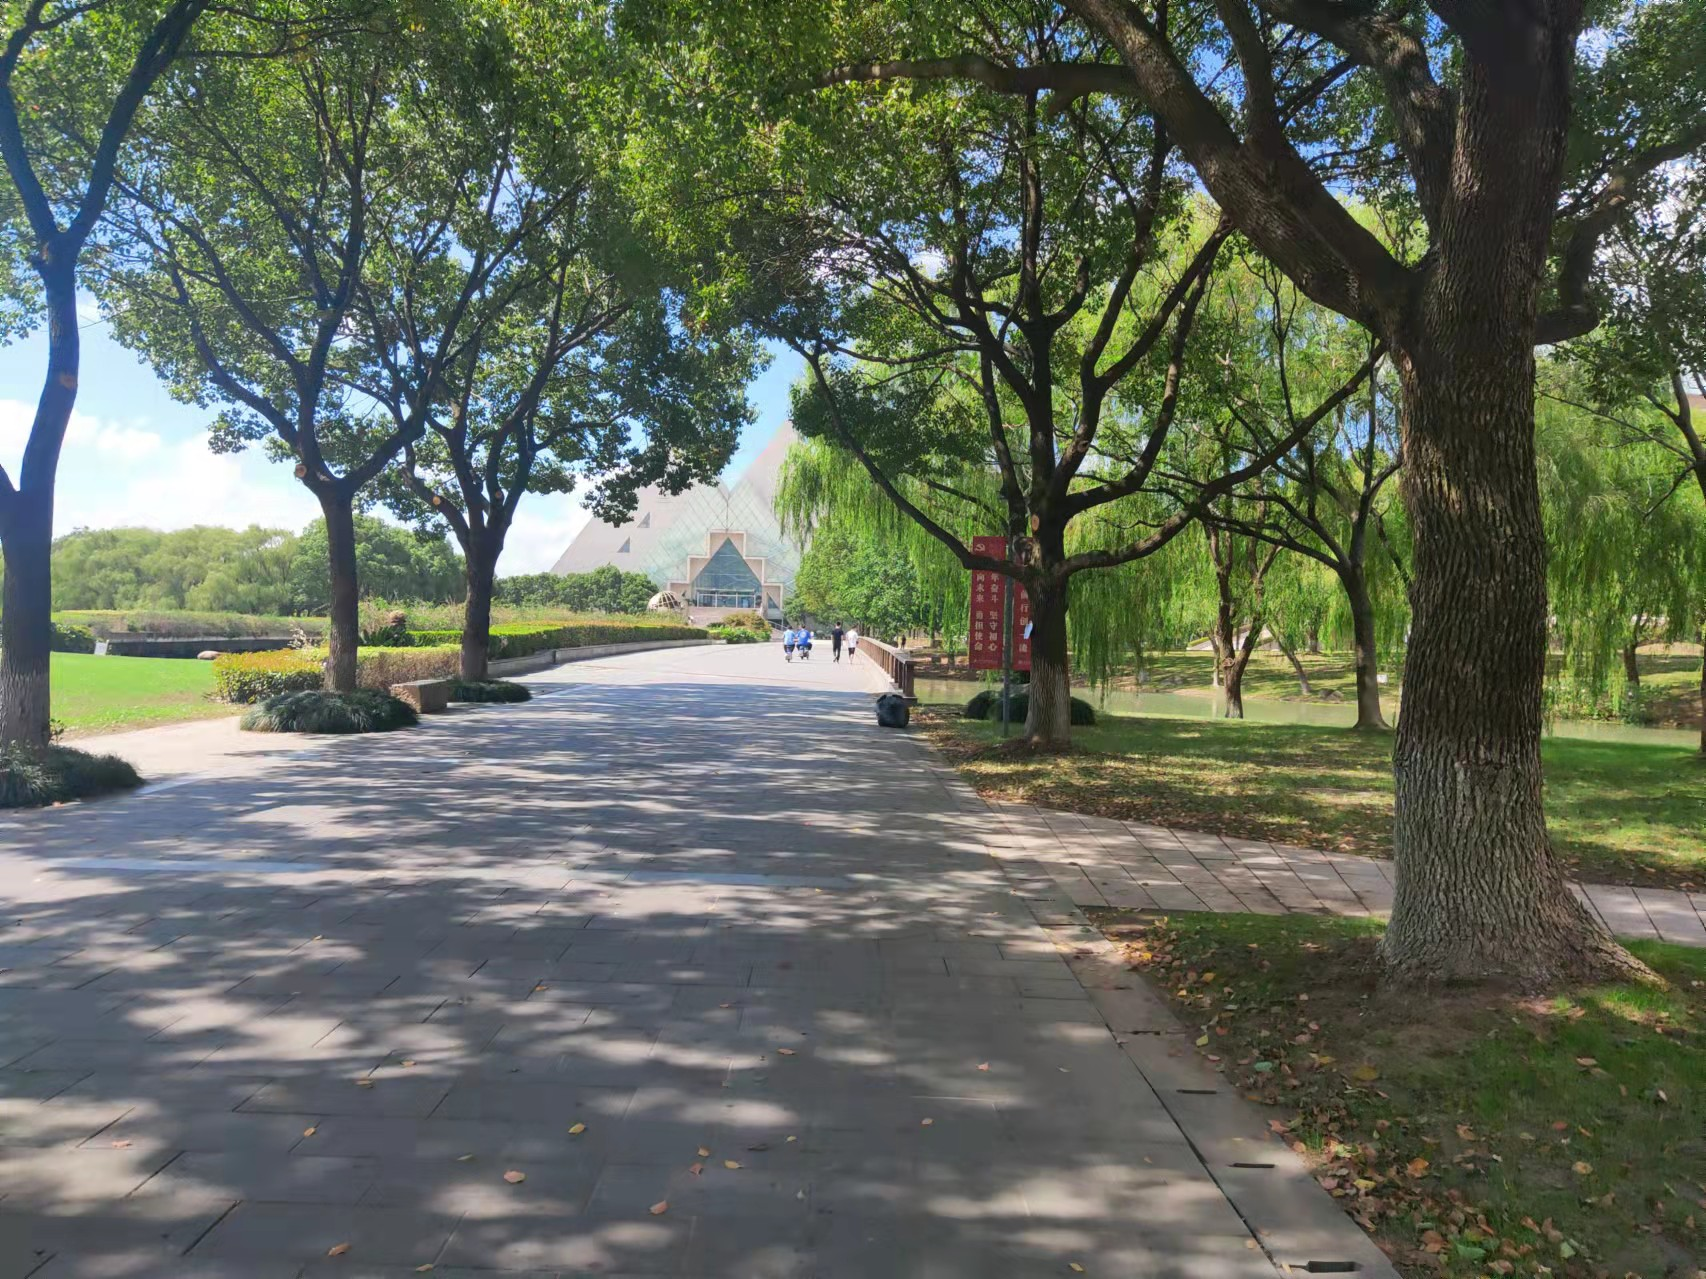
\includegraphics[width=0.6\textwidth]{test.jpg}
                    %\caption{fig1}
                \end{minipage}%
            }%
            \subfigure[RGB模型转YUV模型]{
                \begin{minipage}[t]{0.3\linewidth}
                    \centering
                    \includegraphics[width=0.6\textwidth]{rgb2yuv.jpg}
                    %\caption{fig2}
                \end{minipage}%
            }%
            \subfigure[YUV模型转RGB模型]{
                \begin{minipage}[t]{0.3\linewidth}
                    \centering
                    \includegraphics[width=0.6\textwidth]{yuv2rgb.jpg}
                    %\caption{fig2}
                \end{minipage}%
            }%
            \caption{RGB模型和YUV模型之间的转换}
            \label{fig:fig_rgb_yuv}
        \end{figure}
        \hspace{2em}由图\ref{fig:fig_rgb_yuv}可以看到,转换的结果稍微有些失真,这是由于YUV采样的原因导致的结果。
        \subsubsection{YCbCr模型}
        \hspace{2em}YCbCr模型是对YUV经过缩放和偏移的翻版。其中Y与YUV中的Y含义是一致的,Cb,Cr同样都指的是色彩,只是在表达方式上不同而已.在YUV家族中,YCbCr是在计算机系统中应用最多的成员,其应用领域很广泛,一般人们所讲的大多数指的是YCbCr模型.\\
        \hspace{2em}YCbCr模型与RGB模型相互转换的方式如下所示
        \begin{eqnarray}
            \left[\begin{array}{c}
                Y\\
                Cb\\
                Cr\\
            \end{array}\right]=\left[\begin{array}{ccc}
                0.257 & 0.564 & 0.098\\
                -0.148 & -0.291 & 0.439\\
                0.439 & -0.368 & -0.071\\
            \end{array}\right]\left[\begin{array}{c}
                R\\
                G\\
                B\\
            \end{array}\right]+\left[\begin{array}{c}
               16\\
               128\\
               128\\
            \end{array}\right]\nonumber
        \end{eqnarray}
        \hspace{2em}下面是使用到YCbCr模型与RGB模型之间转换的一个样例:
        \begin{figure}[htbp]
            \centering
            \subfigure[原图像]{
                \begin{minipage}[t]{0.3\linewidth}
                    \centering
                    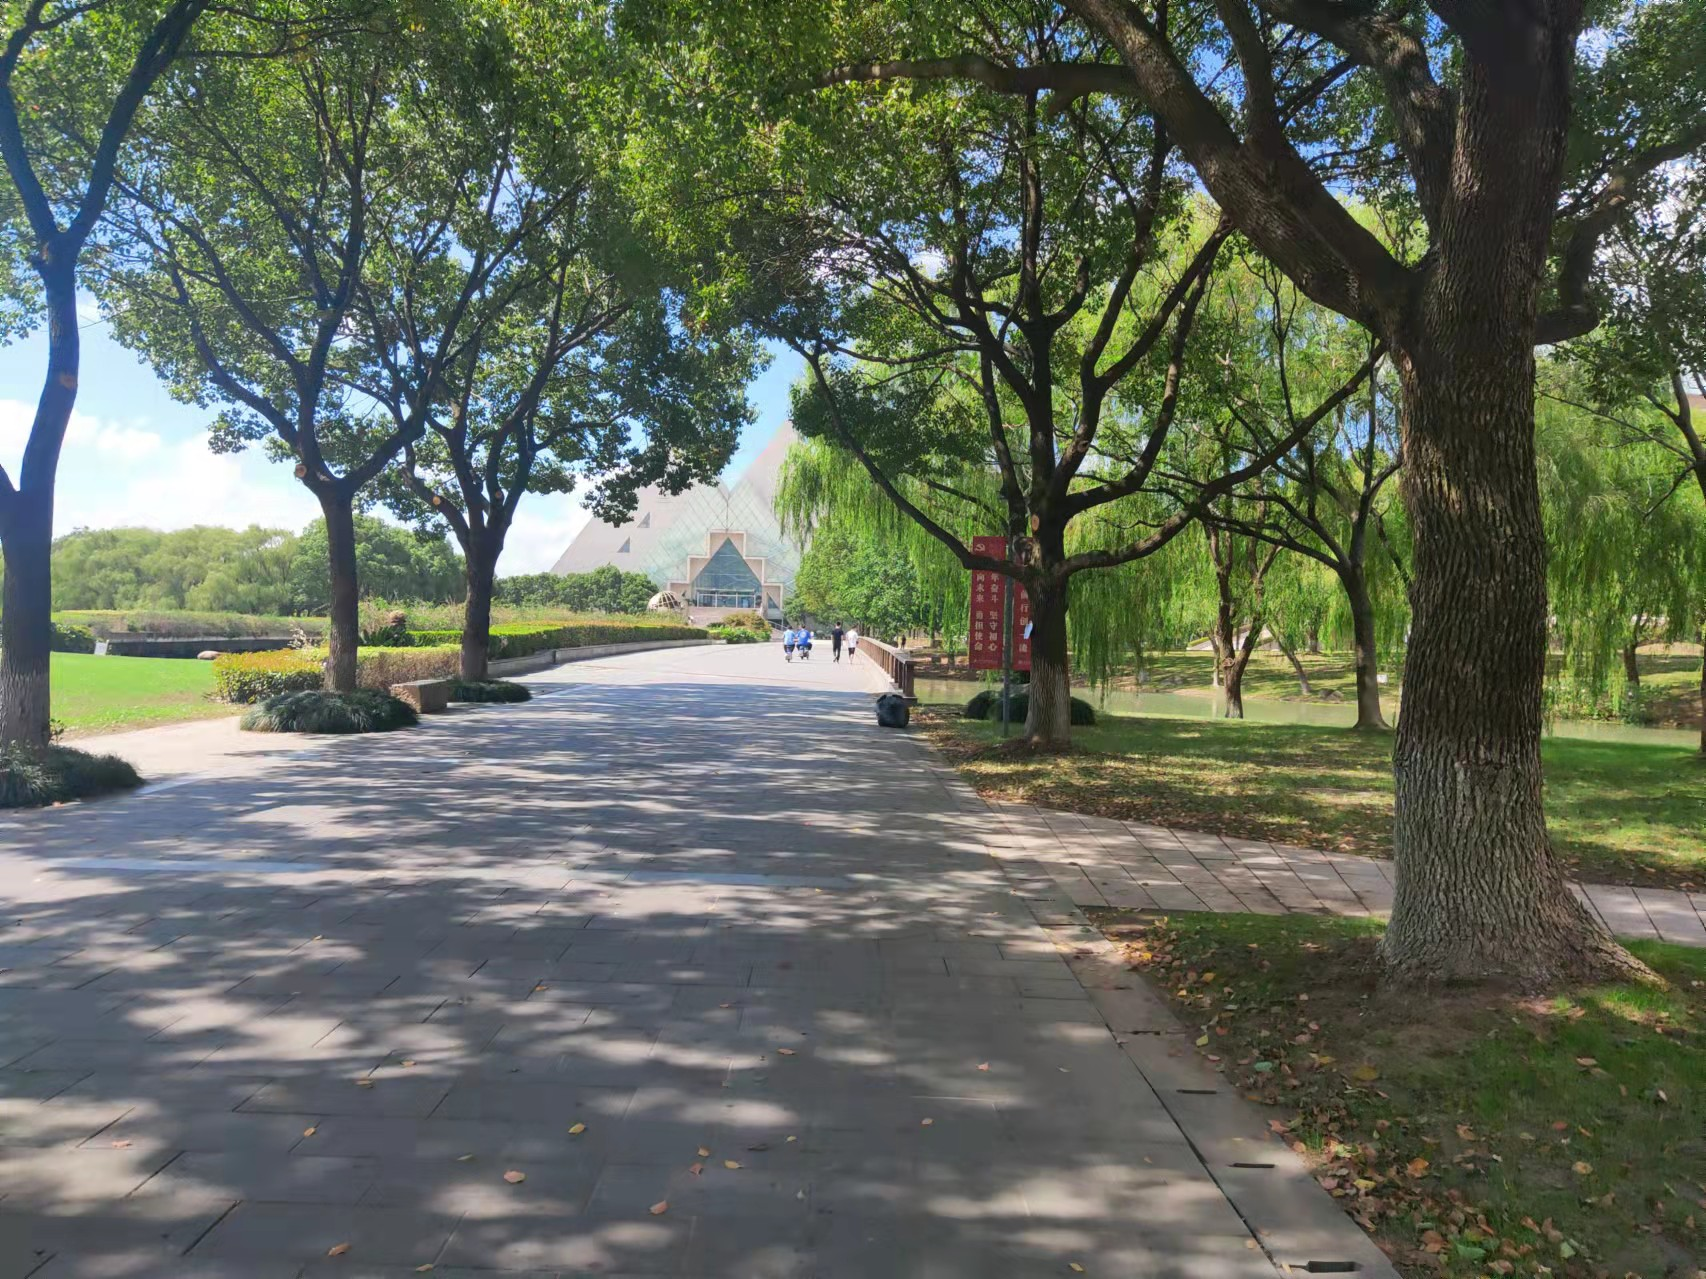
\includegraphics[width=0.6\textwidth]{test.jpg}
                    %\caption{fig1}
                \end{minipage}%
            }%
            \subfigure[RGB模型转YCbCr模型]{
                \begin{minipage}[t]{0.3\linewidth}
                    \centering
                    \includegraphics[width=0.6\textwidth]{rgb2ycbcr.jpg}
                    %\caption{fig2}
                \end{minipage}%
            }%
            \subfigure[YCbCr模型转RGB模型]{
                \begin{minipage}[t]{0.3\linewidth}
                    \centering
                    \includegraphics[width=0.6\textwidth]{ycbcr2rgb.jpg}
                    %\caption{fig2}
                \end{minipage}%
            }%
            \caption{RGB模型和YCbCr模型之间的转换}
            \label{fig:fig_rgb_yuv}
        \end{figure}
        \hspace{2em}图中稍微出现的问题就是,在YCbCr模型转换到RGB模型的时候出现了一些问题。
        \subsection{任务二:HSI图像和HSV图像之间的转换}
        \subsubsection{HSI模型}
        \hspace{2em}RGB模型可以很好地模拟计算机中的彩色模型,但是并不能够很好地适应人实际上解释的颜色。观察彩色物体的时候,我们经常使用到的是色彩的色调、饱和度和亮度来描述这个物体。色调描述的是一种纯色颜色的属性,而饱和度是一种纯色被白光稀释程度的度量。亮度是一个主管描述子,实际上它是不可度量的,它体现的是无色的强度概念,并且是描述色彩感觉的关键因子之一,所以很清楚地知道强度(灰度级)是单色图像中最有用的描述子。\\
        \hspace{2em}HSI模型是从人眼的角度来表示颜色的空间表示和分布,HSI空间由一个垂直强度轴和位于该轴垂直的平面内的彩色轨迹表示。当平面沿强度轴上下移动时候,由每个平面与立方体表面构成的横截面定义的边界不是三角形就是六边形,更一般的可以是圆形的方式。如图\ref{fig:fig_hsi_model}所示\\
        \begin{figure}[htbp]
            \centering
            \subfigure[不同的HSI颜色模型表示的方法]{
                \begin{minipage}[t]{0.3\linewidth}
                    \centering
                    \includegraphics[width=0.95\textwidth]{fig_hsi_shapes.jpg}
                    %\caption{fig1}
                \end{minipage}%
            }%
            \subfigure[三棱锥HSI颜色模型表示方法]{
                \begin{minipage}[t]{0.3\linewidth}
                    \centering
                    \includegraphics[width=0.6\textwidth]{fig_hsi_triangle.jpg}
                    %\caption{fig2}
                \end{minipage}%
            }%
            \subfigure[圆锥HSI颜色模型表示方法]{
                \begin{minipage}[t]{0.3\linewidth}
                    \centering
                    \includegraphics[width=0.6\textwidth]{fig_hsi_circle.jpg}
                    %\caption{fig2}
                \end{minipage}%
            }%
            \caption{HSI模型表示方法}
            \label{fig:fig_hsi_model}
        \end{figure}
        \hspace{2em}HSI模型的建立基于两个重要的事实:第一个就是分量与图像的彩色信息无关;第二个就是H和S分量与人感受颜色的方式是紧密相联的,这些特点使得HSI模型非常适合彩色特性检测与分析.一般HSI表述如下所示
        \begin{itemize}
            \item 色调H(Hue):与光波的频率是有关系的,它表示人的感官对不同颜色的感受,也可以表示一定范围的颜色,例如暖色、冷色等等.
            \item 饱和度S(Saturation):表示颜色的纯度,纯光谱色是完全饱和的,加入白光会稀释饱和度.饱和度越大,颜色看起来就越来越鲜艳,反之亦然.
            \item 亮度I(Intensity):对应成像亮度和图像灰度,是颜色的明亮程度.
        \end{itemize}
        \hspace{2em}HSI色彩空间是从人的视觉系统出发,用色调、色饱和度和亮度来描述色彩的变化。\\
        \heiti\textbf{从RGB到HSI的彩色转换}\songti\\
        
        \hspace{2em}给定一幅RGB彩色格式的图像,每个RGB像素的H分量可以用以下的公式得到:
        \begin{eqnarray}
            H&=&\begin{cases}
                \theta,&B\leq{G}\\
                360-\theta,&B>{G}\\
            \end{cases}\nonumber
        \end{eqnarray}
        上述表达式中有
        \begin{eqnarray}
            \theta&=&\arccos\left\{\dfrac{\frac{1}{2}\left[(R-G)+(R-B)\right]}{\sqrt{(R-G)^2}+(R-B)(G-B)}\right\}\nonumber
        \end{eqnarray}
        \hspace{2em}饱和度分量由下面的公式给出:
        \begin{eqnarray}
            S&=&1-\dfrac{3\min(R,G,B)}{R+G+B}\nonumber
        \end{eqnarray}
        \hspace{2em}最后强度分量由下面的表达式给出
        \begin{eqnarray}
            I&=&\dfrac{1}{3}(R+G+B)\nonumber
        \end{eqnarray}
        
        \hspace{2em}一般来说,HSI三个分量的取值范围分别是$S\in{[0,1]}$,$I\in{[0,255]}$,$H\in{[0,2\pi]}$.\\
        \heiti\textbf{从HSI到RGB的彩色转换}\songti\\
        \hspace{2em}从HSI转换到RGB的时候,稍微些许繁琐,一般地有以下的变换:\\
        \begin{itemize}
            \item RG扇区$\left[0,\dfrac{2\pi}{3}\right]$:当H属于这个扇区的时候,RGB分量由以下的公式给出:
            \begin{eqnarray}
                B&=&I(1-S)\nonumber\\
                R&=&I\left[1+\dfrac{S\cos{H}}{\cos\left(\frac{\pi}{3}-H\right)}\right]\nonumber\\
                G&=&3I-(R+B)\nonumber
            \end{eqnarray}
            \item GB扇区$\left[\dfrac{2\pi}{3},\dfrac{4\pi}{3}\right]$:如果给定的H值在该扇区中,则首先从H中减去$\dfrac{2\pi}{3}$,即
            \begin{eqnarray}
                H&=&H-\dfrac{2\pi}{3}\nonumber
            \end{eqnarray}
            所以这样RGB分量如下所示
            \begin{eqnarray}
                R&=&I(1-S)\nonumber\\
                G&=&I\left[1+\dfrac{S\cos{H}}{\cos\left(\dfrac{\pi}{3}-H\right)}\right]\nonumber\\
                B&=&3I-(R+G)\nonumber
            \end{eqnarray}
            \item BR扇区$\left[\dfrac{2\pi}{3},\dfrac{4\pi}{3}\right]$:最后,如果H的值在该扇区中,则从H中减去$\dfrac{4\pi}{3}$,即
            \begin{eqnarray}
                H&=&H-\dfrac{4\pi}{3}\nonumber
            \end{eqnarray}
            则RGB分量如下所示
            \begin{eqnarray}
                G&=&I(1-S)\nonumber\\
                B&=&I\left[1+\dfrac{S\cos{H}}{\cos\left(\dfrac{\pi}{3}-H\right)}\right]\nonumber\\
                R&=&3I-(G+B)\nonumber
            \end{eqnarray}
        \end{itemize}
        \hspace{2em}HSI模型与RGB模型效果图如下图所示
        \begin{figure}[htbp]
            \centering
            \subfigure[原图像]{
                \begin{minipage}[t]{0.3\linewidth}
                    \centering
                    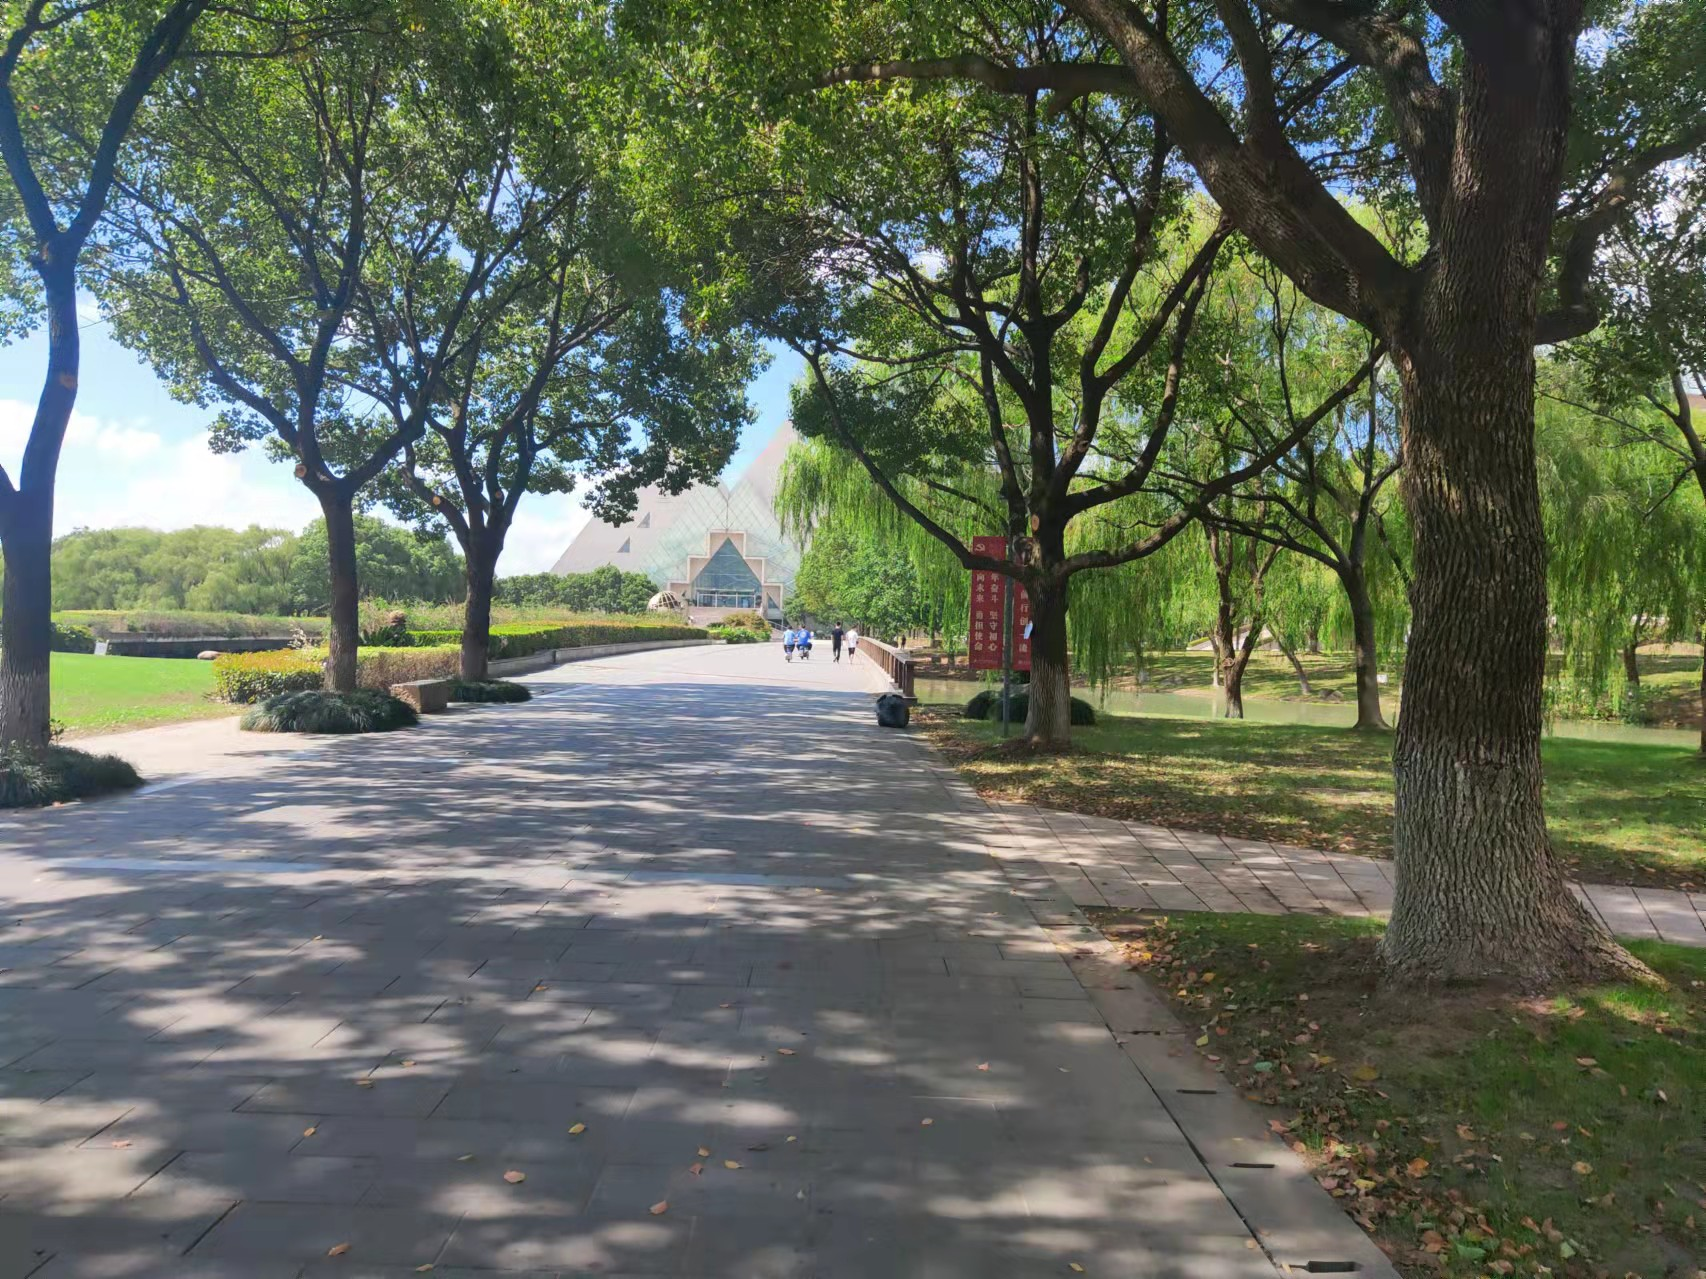
\includegraphics[width=0.95\textwidth]{test.jpg}
                    %\caption{fig1}
                \end{minipage}%
            }%
            \subfigure[RGB转HSI(以HSI模式显示)]{
                \begin{minipage}[t]{0.3\linewidth}
                    \centering
                    \includegraphics[width=0.95\textwidth]{rgb2hsi.jpg}
                    %\caption{fig2}
                \end{minipage}%
            }%
            \subfigure[HSI转RGB(以RGB模式显示)]{
                \begin{minipage}[t]{0.3\linewidth}
                    \centering
                    \includegraphics[width=0.95\textwidth]{hsi2rgb.jpg}
                    %\caption{fig2}
                \end{minipage}%
            }%
            \caption{RGB模型与HSI模型之间相互转换}
            \label{fig:fig_rgb_hsi_model}
        \end{figure}
        \subsubsection{HSV模型}
        \hspace{2em}另外一种在图像处理上使用比较多的是HSV颜色空间,它比RGB更加接近人们对彩色的感知经验,非常直观地表达颜色的色调、鲜艳程度,方便进行颜色的对比。特别地,在HSV颜色空间下,比RGB颜色模型更加容易跟踪某种颜色的物体,常常用于分割指定颜色的物体。\\
        \hspace{2em}通常来讲,HSV表达彩色图像的方式由以下的三个部分组成:
        \begin{itemize}
            \item Hue(色调、色相);
            \item Saturation(饱和度、色彩纯净度);
            \item Value(明度).
        \end{itemize}
        \hspace{2em}图\ref{fig:fig_hsv}使用到的是一个非常形象化描述的一个HSV颜色空间,圆柱体的横截面可以看做是一个极坐标系,H用极坐标系的极角表示,S用极坐标系的极轴长度表示,V用圆柱中的高度表示.\\
        \begin{figure}[hbpt]
            \centering
            \includegraphics[width=0.28\textwidth]{fig_hsv.jpg}
            \caption{HSV颜色模型}
            \label{fig:fig_hsv}
        \end{figure}
        \heiti\textbf{从RGB到HSV的彩色转换}\songti\\
        \hspace{2em}现在设$c_{\max}=\max(R,G,B),c_{\min}=\min(R,G,B),\Delta=c_{\max}-c_{\min}$那么,转换的方式如下所示\\
        \begin{eqnarray}
            H&=&\begin{cases}
                0,&\Delta=0\\
                \frac{\pi}{3}\cdot\frac{G-B}{\Delta},&c_{\max}=R\\
                \frac{\pi}{3}\cdot\frac{G-B}{\Delta}+\frac{2\pi}{3},&c_{\max}=G\\
                \frac{\pi}{3}\cdot\frac{G-B}{\Delta}+\frac{4\pi}{3},&c_{\max}=B 
            \end{cases}\nonumber\\
            S&=&\begin{cases}
                0,&c_{\max}=0\\
                \dfrac{\Delta}{c_{\max}},&c_{\max}\neq{0}\\
            \end{cases}\nonumber\\
            V&=&c_{\max}\nonumber
        \end{eqnarray}
        很多模型中,一般情况下使用的是角度值进行度量而不是用弧度制进行度量。\\
        \heiti\textbf{从HSV到RGB的彩色转换}\songti\\
        \hspace{2em}设
        \begin{eqnarray}
            h&=&\left\lfloor\dfrac{H}{60}\right\rfloor\mod{6}\nonumber\\
            f&=&\dfrac{H}{60}-h\nonumber\\
            p&=&v\cdot(1-s)\nonumber\\
            q&=&v\cdot{(1-f\cdot{s})}\nonumber\\
            t&=&v\cdot(1-(1-f)\cdot{s})\nonumber
        \end{eqnarray}
        转换的公式如下所示
        \begin{eqnarray}
            (r,g,b)&=&\begin{cases}
                (v,t,p),&h=0\\
                (q,v,p),&h=1\\
                (p,v,t),&h=2\\
                (p,q,v),&h=3\\
                (t,p,v),&h=4\\
                (v,p,q),&h=5
            \end{cases}\nonumber
        \end{eqnarray}
        转换的结果如下所示
        \begin{figure}[htbp]
            \centering
            \subfigure[原图像]{
                \begin{minipage}[t]{0.3\linewidth}
                    \centering
                    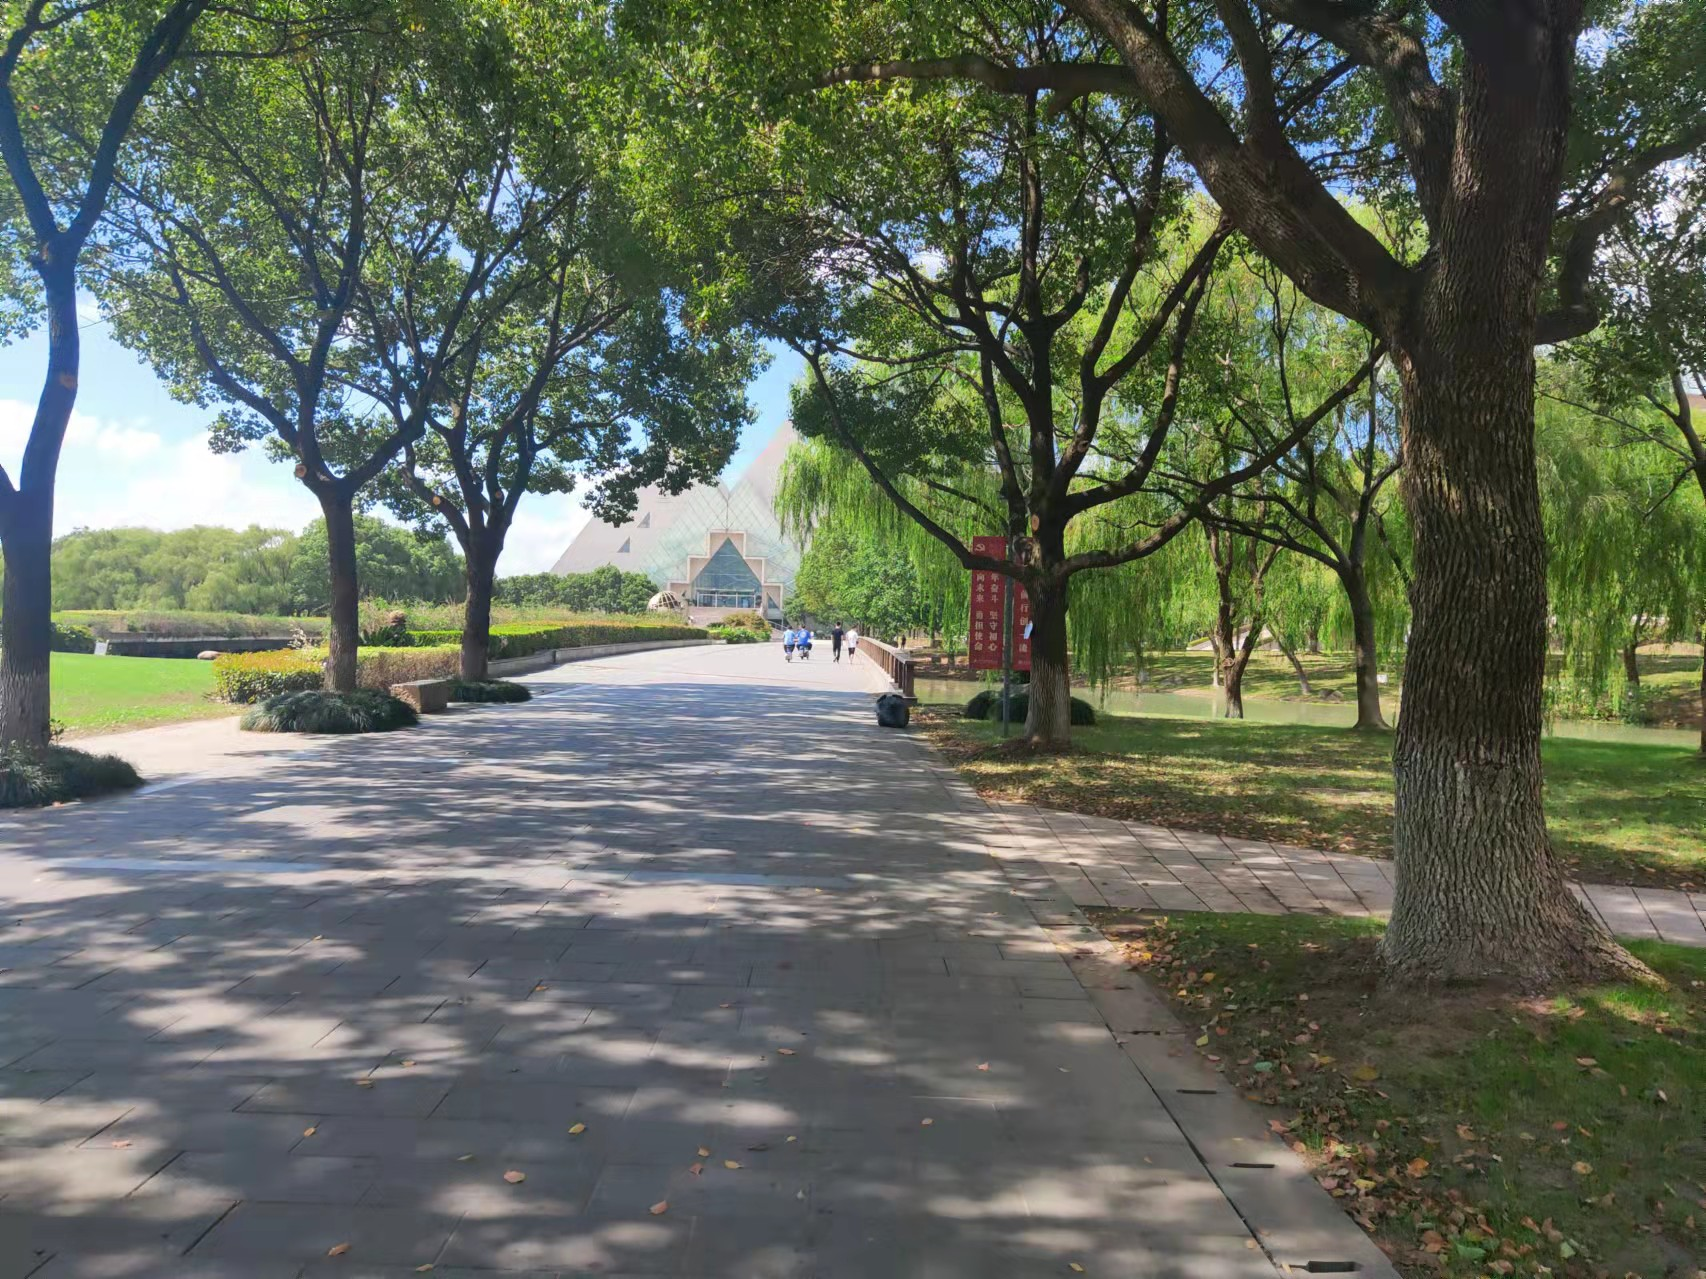
\includegraphics[width=0.95\textwidth]{test.jpg}
                    %\caption{fig1}
                \end{minipage}%
            }%
            \subfigure[RGB转HSV(以HSV模式显示)]{
                \begin{minipage}[t]{0.3\linewidth}
                    \centering
                    \includegraphics[width=0.95\textwidth]{rgb2hsv.jpg}
                    %\caption{fig2}
                \end{minipage}%
            }%
            \subfigure[HSV转RGB(以RGB模式显示)]{
                \begin{minipage}[t]{0.3\linewidth}
                    \centering
                    \includegraphics[width=0.95\textwidth]{hsv2rgb.jpg}
                    %\caption{fig2}
                \end{minipage}%
            }%
            \caption{RGB模型与HSV模型之间相互转换}
            \label{fig:fig_rgb_hsv_model}
        \end{figure}
        \subsection{任务三:提取灰度分量进行直方图均衡化与规定化}
        \subsubsection{灰度图像的直方图均衡化}
        \hspace{2em}灰度级别范围为$[0,L-1]$的数字图像的直方图是离散函数$h(r_{k})=n_{k}$,其中$r_{k}$是第$k$季度灰度值,$n_{k}$是图像中灰度为$r_{k}$的像素个数.通过直方图增强技术可以使得灰度值分布不均匀的图像通过直方图均衡化之后将灰度值的分布变得更加均匀.\\
        \hspace{2em}现在我们考虑到的是连续灰度值,并且用$r$表示待处理的图像灰度值,假设$r$的取值区间范围为$[0,L-1]$,并且$0$表示的是黑色,$r=L-1$表示的是白色.在$r$满足这些条件的情况下,我们将注意力几种在变换形式
        \begin{eqnarray}
            s&=&T(r).0\leq{r}\leq{L-1}\nonumber
        \end{eqnarray}
        上灰度映射,对于输入图像找那个每个具有$r$值的像素产生一个输出灰度值s,我们假设这样的函数满足以下的条件
        \begin{itemize}
            \item $T(r)$在区间$0\leq{r}\leq{L-1}$上为单调递增函数;
            \item 当$0\leq{r}\leq{L-1}$时候,$0\leq{T(r)}\leq{L-1}$.
        \end{itemize}
        \hspace{2em}一幅图像的灰度级可以视为区间$[0,L-1]$上的随机变量.随机变量的基本描绘子是其概率密度函数.若$p_{r}(r),p_{s}(s)$分别表示的是随机变量$r,s$概率密度函数,其中$p$下标表示的是不同的概率密度函数.一般变化之后的变量s通过以下的公式可以得到
        \begin{eqnarray}
            p_{s}(s)&=&p_{r}(r)\left|\dfrac{dr}{ds}\right|\nonumber
        \end{eqnarray}
        所以这样就会得到在图像处理中,特别重要的变换函数
        \begin{eqnarray}
            s&=&T(r)=(L-1)\int_{0}^{r}p_{r}(w)dw\nonumber
        \end{eqnarray}
        上式中,$w$是积分的假变量,公式的右边是随机变量$r$的累积分布函数(CDF).这就是直方图均衡化的基本数学模型.\\
        \hspace{2em}对于离散值,我们处理其概率(直方图值)与求和来替代处理概率密度函数与积分,一幅数字图像中灰度级$r_{k}$出现的概率近似为
        \begin{eqnarray}
            p_{r}(r_{k})&=&\dfrac{n_{k}}{MN},k=0,1,2,\dots,L-1\nonumber
        \end{eqnarray}
        上述表达式中,$MN$是图像的总像素,$n_{k}$是灰度为$r_{k}$的像素个数,$L$是图像中可能灰度级的数量.与$r_{k}$相对的$p_{k}(r_{k})$图像通常称为直方图.
        故而离散的形式表达为以下的形式:
        \begin{eqnarray}
            s_{k}&=&T(r_{k})=(L-1)\sum\limits_{j=0}^{k}p_{r}(r_{j})=\dfrac{L-1}{MN}\sum\limits_{j=0}^{k}n_{j},k=0,1,2,\dots,L-1\nonumber
        \end{eqnarray}
        所以这样就会将原来输入图像中灰度值为$r_{k}$的图像变换为输出图像中灰度值为$s_{k}$的对应像素,这个公式中变换映射$T(r_{k})$一般称为直方图均衡或者是直方图线性变换.\\

        \hspace{2em}下面我们使用一幅灰度图像进行实验处理.通过以下的灰度计算公式可以得到
        \begin{eqnarray}
            \text{Gray}&=&0.299*R+0.587*G+0.114*B\nonumber
        \end{eqnarray}
        我们对灰度图像进行直方图均衡化处理可以得到以下的图像,如图\ref{fig:fig_gray_hist_imporve_model}所示:\\
        \begin{figure}[htbp]
            \centering
            \subfigure[原图像]{
                \begin{minipage}[t]{0.3\linewidth}
                    \centering
                    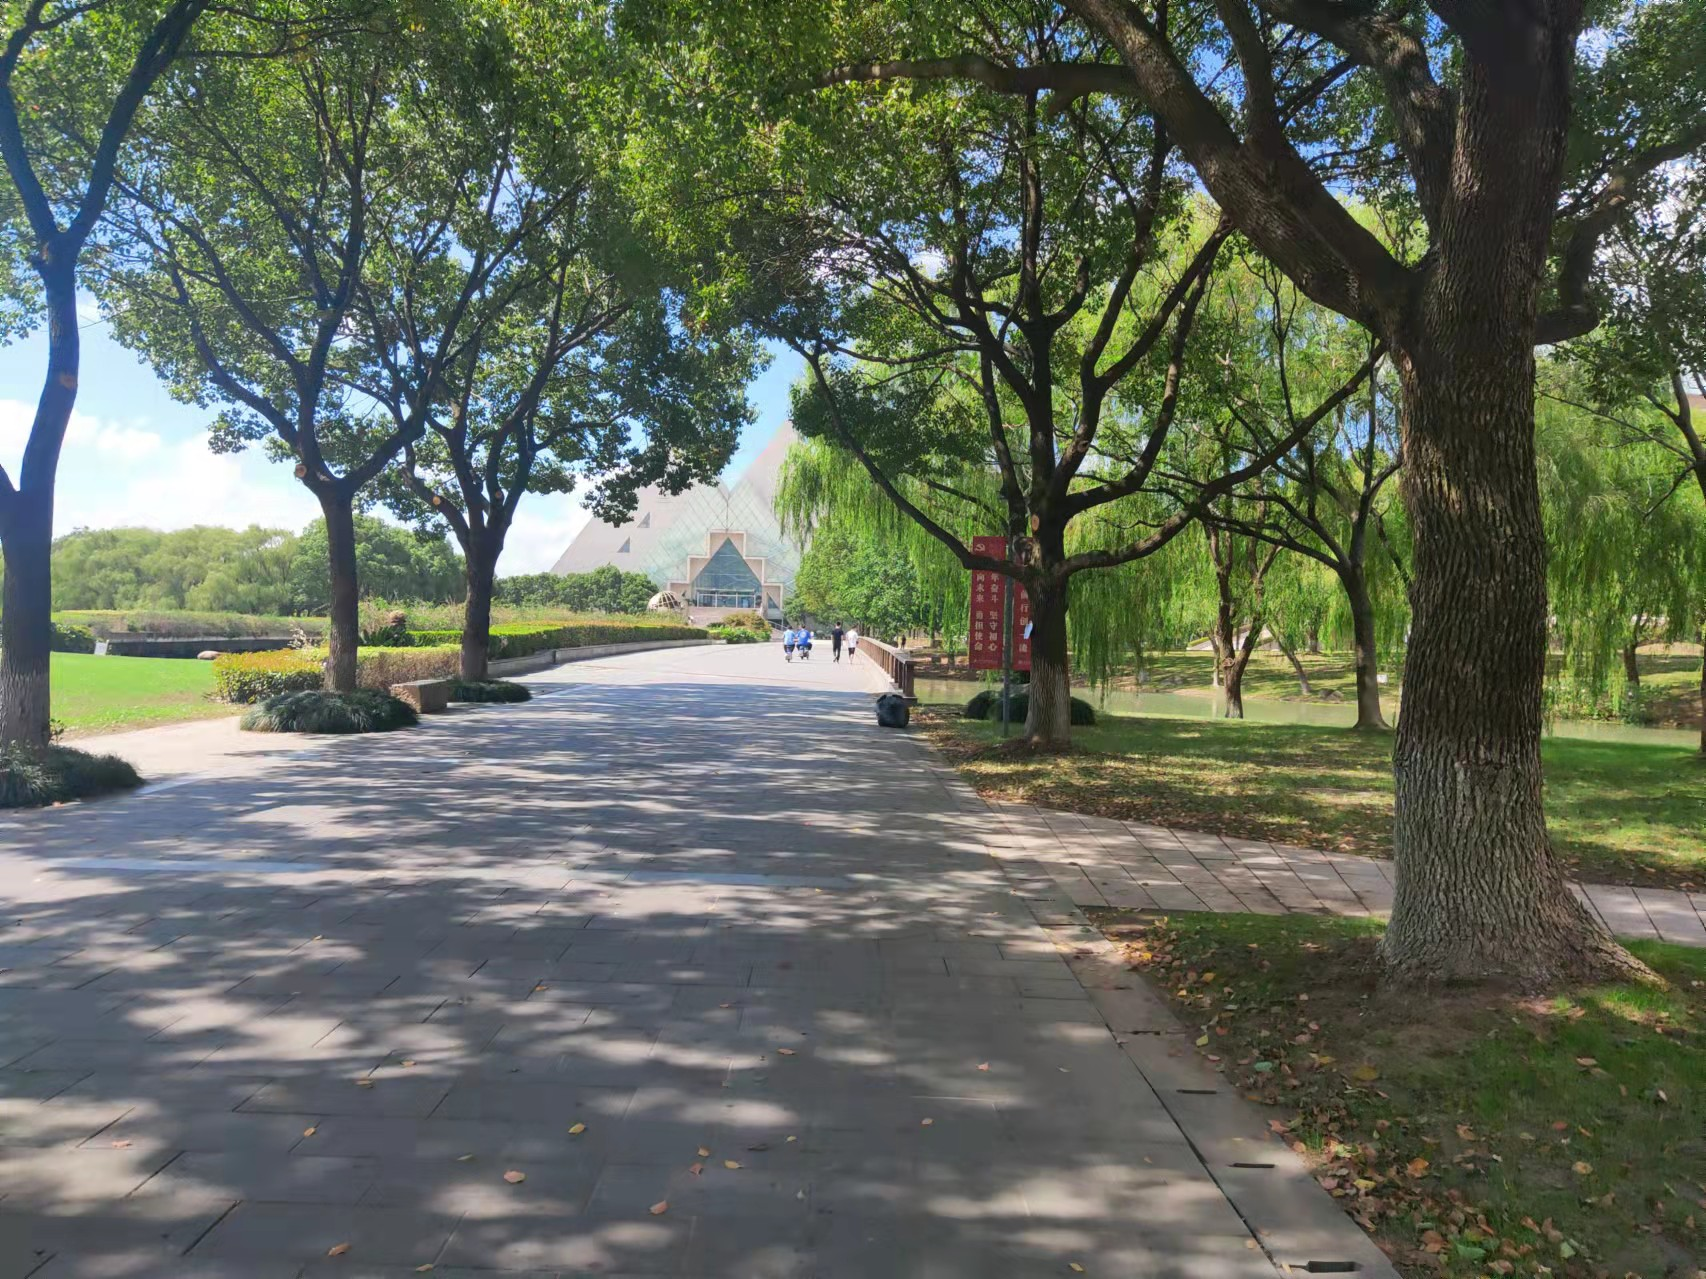
\includegraphics[width=0.95\textwidth]{test.jpg}
                    %\caption{fig1}
                \end{minipage}%
            }%
            \subfigure[灰度图像(灰度公式转换得到)]{
                \begin{minipage}[t]{0.3\linewidth}
                    \centering
                    \includegraphics[width=0.95\textwidth]{rgb2gray.jpg}
                    %\caption{fig2}
                \end{minipage}%
            }%
            \subfigure[直方图增强后的灰度图像]{
                \begin{minipage}[t]{0.3\linewidth}
                    \centering
                    \includegraphics[width=0.95\textwidth]{gray_improved.jpg}
                    %\caption{fig2}
                \end{minipage}%
            }%
            \caption{RGB模型与HSV模型之间相互转换}
            \label{fig:fig_gray_hist_imporve_model}
        \end{figure}
        \newpage
        \hspace{2em}对比原图来说,我们明显可以看到,直方图增强之后的图片更加清晰,但是同时直方图增强的方法使得图片的亮度增高,这是直方图最大的一个问题.下面图\ref{fig:fig_gray_hist_cdf_before_after}是直方图增强之前和之后的概率密度分布图像.\\
        \begin{figure}[htbp]
            \centering
            \subfigure[原始概率分布]{
                \begin{minipage}[t]{0.5\linewidth}
                    \centering
                    \includegraphics[width=0.95\textwidth]{hist_before.png}
                    %\caption{fig1}
                \end{minipage}%
            }%
            \subfigure[原始累计函数分布]{
                \begin{minipage}[t]{0.5\linewidth}
                    \centering
                    \includegraphics[width=0.95\textwidth]{cdf_hist_before.png}
                    %\caption{fig2}
                \end{minipage}%
            }%
            \quad
            \subfigure[直方图增强后的概率分布]{
                \begin{minipage}[t]{0.5\linewidth}
                    \centering
                    \includegraphics[width=0.95\textwidth]{hist_after.png}
                    %\caption{fig2}
                \end{minipage}%
            }%
            \subfigure[直方图增强后的累积分布]{
                \begin{minipage}[t]{0.5\linewidth}
                    \centering
                    \includegraphics[width=0.95\textwidth]{cdf_hist_after.png}
                    %\caption{fig2}
                \end{minipage}%
            }%
            \caption{直方图灰度值统计图}
            \label{fig:fig_gray_hist_cdf_before_after}
        \end{figure}
        \hspace{2em}从图中可以看出,上述四幅图片展示的是直方图均衡之后的直方图以及累计分布,很明显,变换之后的灰度值分布更加均匀一些,累计分布变换变为线性的形式,表明输入的映射为近似相等的输出.尽管这些直方图不同,但是直方图均衡之后的图像本身在视觉上是非常相似的.上述例子表明了直方图均衡作为自适应对比度增强具有一定的作用.
        \subsubsection{灰度图像的规定化}
        \hspace{2em}直方图虽然能够自动地确定变换函数,该函数寻求产生有均匀直方图的输出图像.需要自动增强的时候,这是一种好的方法,因为由这种技术得到的结果可以预知,并且这种方法实现起来也是非常简单的.但是对于某些应用中,采用这种均匀的直方图增强并不是最好的处理方法.有时候我们希望处理后的图像能够通过自己规定的直方图分布可能更加有用,这种用于产生处理后有特殊直方图的方法称为直方图匹配或者是称为直方图规定化.\\
        \hspace{2em}设变换前灰度值为$r$,变换之后的灰度值为$z$,那么并假设$p_{r}(r),p_{z}(z)$分别表示它们所对应的连续概率密度函数.在这种表示方法中,$r$和$z$分别表示输入图像和输出图像的灰度级别.现在可以由给定的输入图像的估计$p_{r}(r)$,而$p_{z}(z)$是我们希望输出图像所具有的指定概率密度函数.\\
        \hspace{2em}令$s$是一个具有以下特性的随机变量
        \begin{eqnarray}
            s&=&T(r)=(L-1)\int_{0}^{r}p_{r}(w)dw\nonumber
        \end{eqnarray}
        上述表达式中,w为积分家变量,这个表达式其实就是直方图均衡的连续形式.\\
        \hspace{2em}定义一个具有以下特性的随机变量$z$:
        \begin{eqnarray}
            G(z)&=&(L-1)\int_{0}^{z}p_{z}(t)dt=s\nonumber
        \end{eqnarray}
        上市表达式中,$t$表示的是积分假变量.由这两个等式相等可以得到
        \begin{eqnarray}
            z&=&G^{-1}\left[T(r)\right]=G^{-1}(s)\nonumber
        \end{eqnarray}
        \hspace{2em}所以只要输入图像估计出$p_{r}(r)$,以及输出图像的分布$p_{z}(z)$,就可以得到变换函数$T(r)$.但是在实践中是非常困难寻找到函数$T(r),G^{-1}$有意义的表达式.但是图像处理中这是离散化表示的,所以在处理离散化问题的数据时候,这种计算方法大大简化.我们可以假设\\
        \begin{eqnarray}
            s_{k}&=&T(r_{k})=(L-1)\sum\limits_{j=0}^{k}p_{r}(r_{j})=\dfrac{L-1}{MN}\sum\limits_{j=0}^{k}n_{j},k=0,1,2,\dots,L-1\label{equ:s_formual}
        \end{eqnarray}
        与上面的表达式是一致的,上述表达式中$MN$是图像的像素总数,$n_{j}$是具有灰度值$r_{j}$的像素数量,$L$是图像中可能的灰度级数量.同样给定一个规定的$s_{k}$值,上述表达式中的离散形式涉及计算变换函数
        \begin{eqnarray}
            G(z_{q})=(L-1)\sum\limits_{i=0}^{q}p_{z}(z_{i})\label{equ:G_q_formual}
        \end{eqnarray}
        对于每一个$q$值,均有
        \begin{eqnarray}
            G(z_{q})&=&s_{k}\nonumber
        \end{eqnarray}
        上述表达式中,$p_{z}(z_{i})$是规定直方图的第$i$个值.与前面一样,我们使用反变换找到了对应期望的值$z_{q}$:
        \begin{eqnarray}
            z_{q}&=&G^{-1}(s_{k})\nonumber
        \end{eqnarray}
        也就是说,上述操作对于每个$s$值给出一个$z$值;这样就形成了从$s$到$z$的一个映射关系.\\
        \hspace{2em}综上所述,直方图规定划的步骤过程如下所示:
        \begin{enumerate}
            \item 计算给定直方图的$p_{r}(r)$,并且用它寻找其表达式\ref{equ:s_formual}直方图的均衡变换.将$s_{k}$四舍五入为范围$[0,L-1]$之内的整数.
            \item 对表达式\ref{equ:G_q_formual},$q=0,1,2,\dots,L-1$计算变换函数$G$的所有值.其中$p_{z}(z_{i})$是规定直方图的值.将$G$的值四舍五入为$[0,L-1]$范围内的整数.将$G$的值存储在一个表当中.
            \item 对于每一个值$s_{k},k=0,1,2,3,\dots,L-1$,使用步骤2中存储的G值寻找相对应的$z_{q}$值,以使得$G(z_{q})$最接近$s_{k}$,并且存储这些从$s$到$z$的映射.当满足给定$s_{k}$的$z_{q}$值多于1的时候(映射不是唯一的),选择最小值.
            \item 先对图像均衡,然后使用步骤3中找到的映射将该图像中每个均衡之后的像素值$s_{k}$映射为直方图规定划之后的图像中的相应$z_{q}$值,形成直方图规定划之后的图像.如果是连续情况,均衡输入图像的中间步骤是概念上的.
        \end{enumerate}
        \hspace{2em}我们通过一个具体的例子对灰度图像进行直方图均衡化处理.我们选择的图像如下所示,参考规定化图像如图\ref{fig:fig_test_refertest}所示\\
        \begin{figure}[htbp]
            \centering
            \subfigure[原始图像]{
                \begin{minipage}[t]{0.38\linewidth}
                    \centering
                    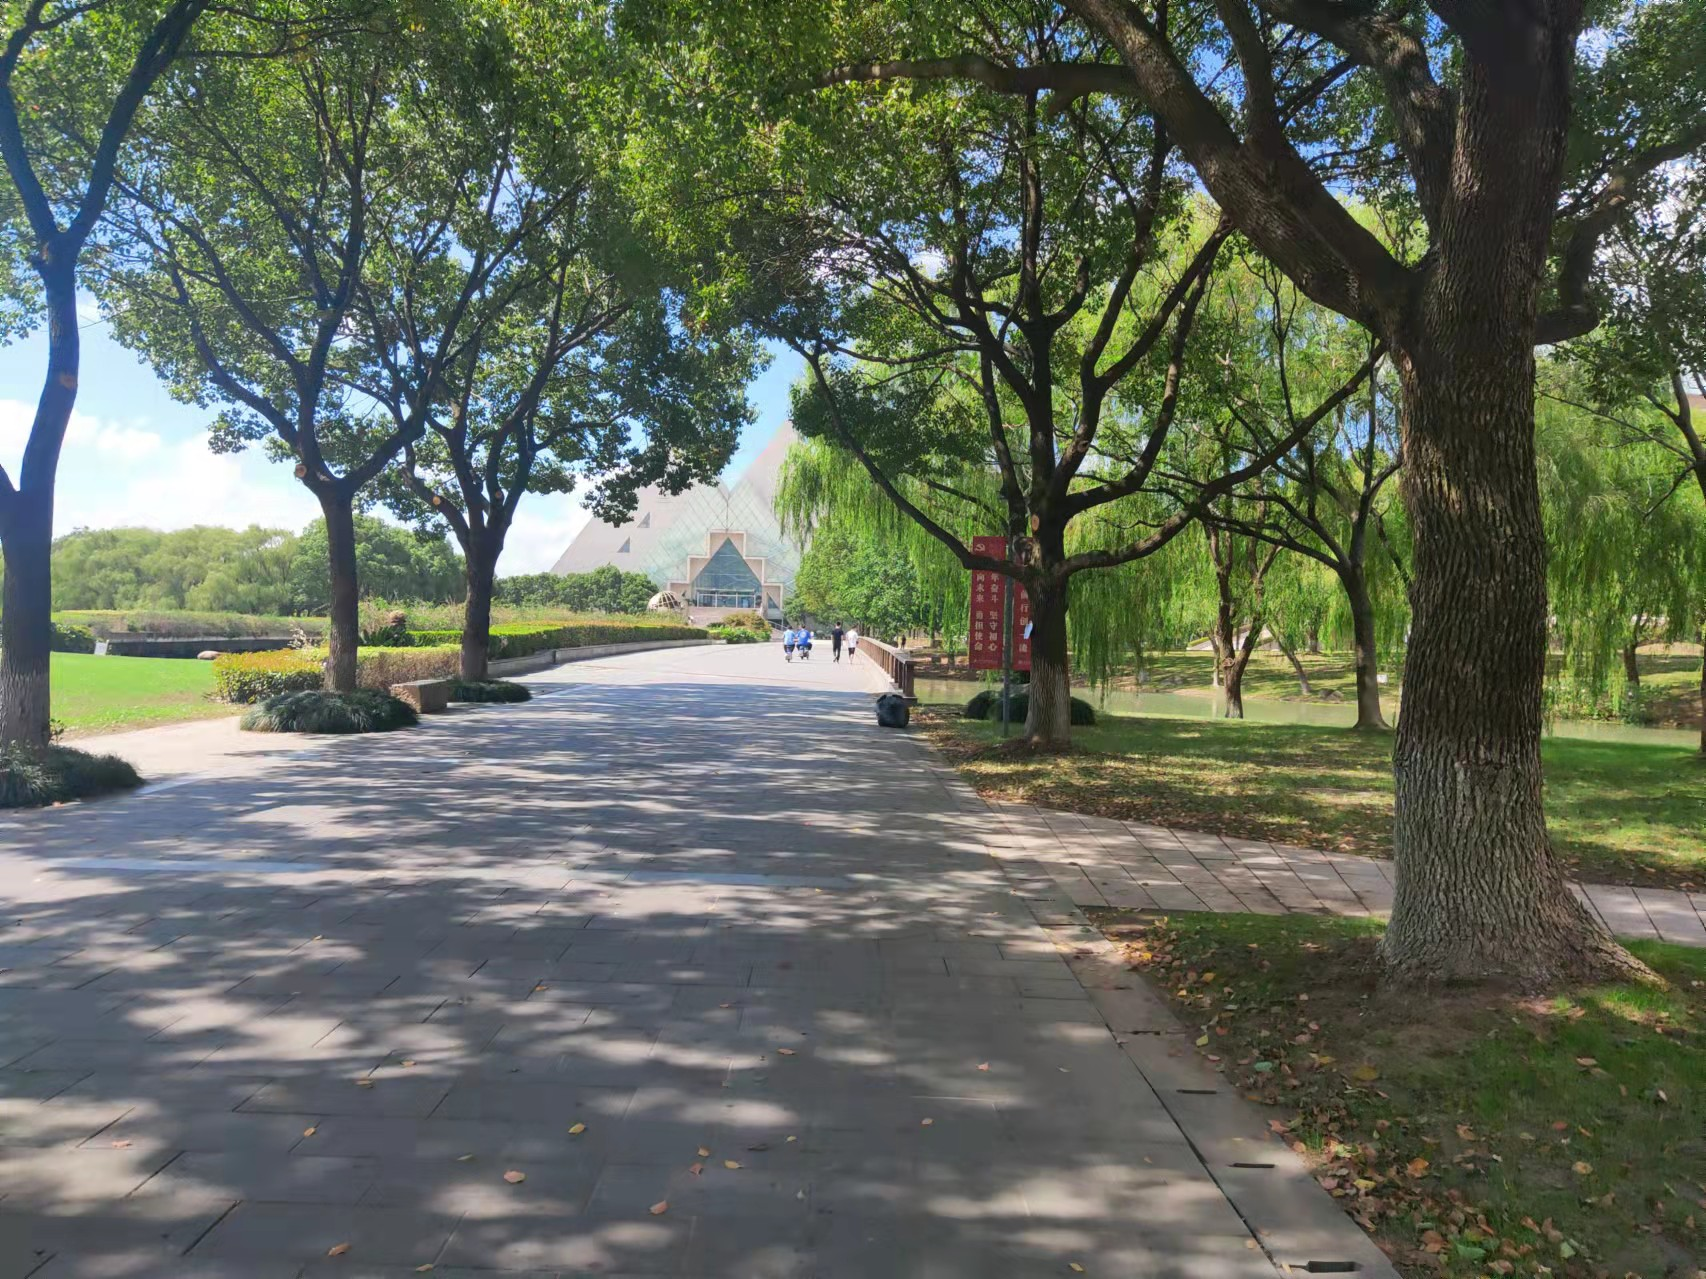
\includegraphics[width=0.95\textwidth]{test.jpg}
                    %\caption{fig1}
                \end{minipage}%
            }%
            \subfigure[参考图像]{
                \begin{minipage}[t]{0.5\linewidth}
                    \centering
                    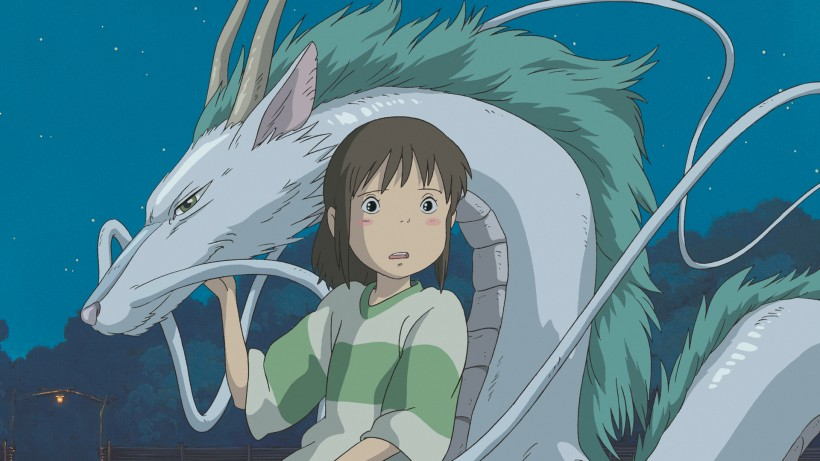
\includegraphics[width=0.95\textwidth]{test1.jpg}
                    %\caption{fig2}
                \end{minipage}%
            }%
            \caption{两幅不同的图像表示}
            \label{fig:fig_test_refertest}
        \end{figure}



        \begin{figure}[htbp]
            \centering
            \subfigure[原始概率分布]{
                \begin{minipage}[t]{0.5\linewidth}
                    \centering
                    \includegraphics[width=0.95\textwidth]{hist_before.png}
                    %\caption{fig1}
                \end{minipage}%
            }%
            \subfigure[原始累计函数分布]{
                \begin{minipage}[t]{0.5\linewidth}
                    \centering
                    \includegraphics[width=0.95\textwidth]{cdf_hist_before.png}
                    %\caption{fig2}
                \end{minipage}%
            }%
            \quad
            \subfigure[参考图像概率密度灰度分布]{
                \begin{minipage}[t]{0.5\linewidth}
                    \centering
                    \includegraphics[width=0.95\textwidth]{hist_before.png}
                    %\caption{fig1}
                \end{minipage}%
            }%
            \subfigure[参考图像累积灰度分布]{
                \begin{minipage}[t]{0.5\linewidth}
                    \centering
                    \includegraphics[width=0.95\textwidth]{cdf_hist_before.png}
                    %\caption{fig2}
                \end{minipage}%
            }%
            \caption{灰度分布图}
            \label{fig:fig_gray_hist_cdf_test_refer}
        \end{figure}
        \hspace{2em}我们对上一步图像进行规定化处理之后得到的对应图像如下图\ref{fig:fig_gray_hist_regularation_imporve_model}所示\\
        \begin{figure}[htbp]
            \centering
            \subfigure[原图像]{
                \begin{minipage}[t]{0.25\linewidth}
                    \centering
                    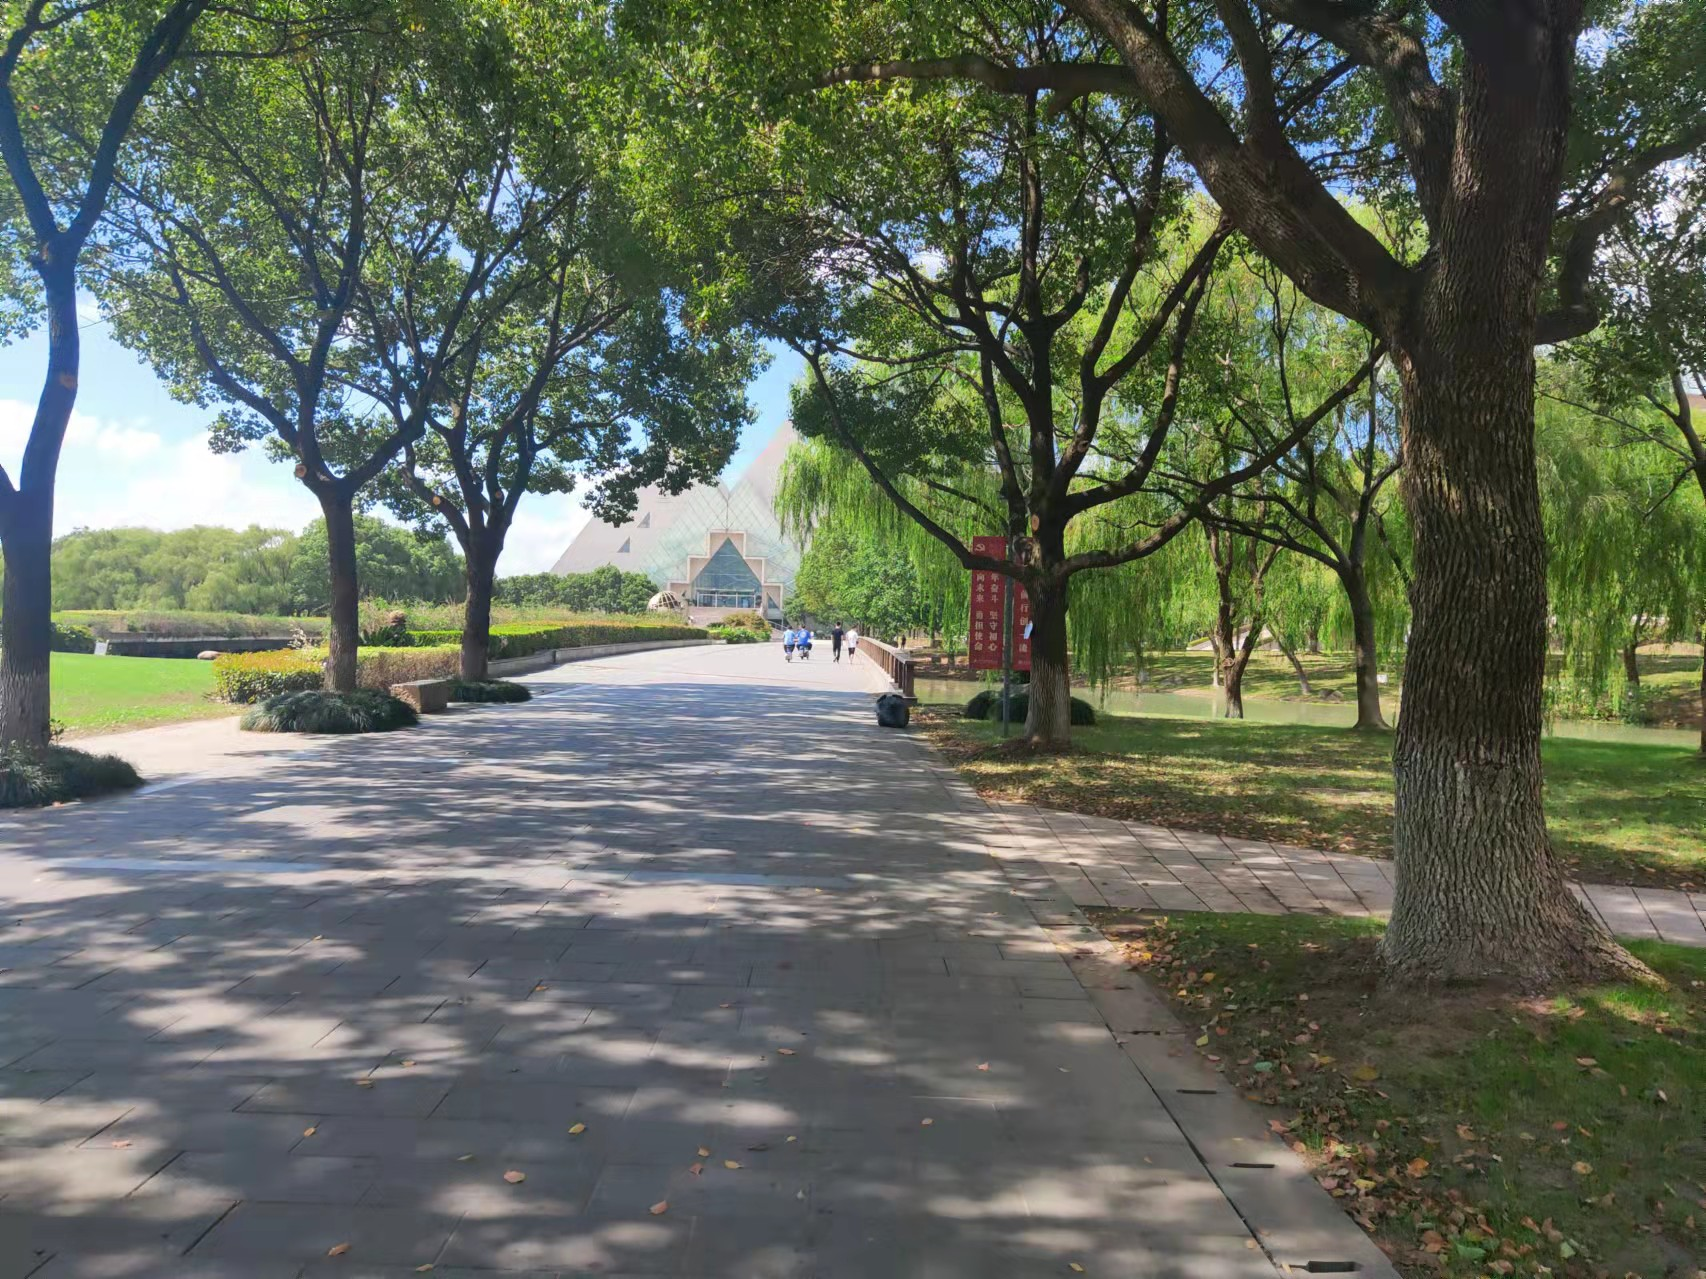
\includegraphics[width=0.95\textwidth]{test.jpg}
                    %\caption{fig1}
                \end{minipage}%
            }%
            \subfigure[灰度图像(灰度公式转换得到)]{
                \begin{minipage}[t]{0.25\linewidth}
                    \centering
                    \includegraphics[width=0.95\textwidth]{rgb2gray.jpg}
                    %\caption{fig2}
                \end{minipage}%
            }%
            \subfigure[直方图均衡化后的灰度图像]{
                \begin{minipage}[t]{0.25\linewidth}
                    \centering
                    \includegraphics[width=0.95\textwidth]{gray_improved.jpg}
                    %\caption{fig2}
                \end{minipage}%
            }%
            \subfigure[直方图规定化化后的灰度图像]{
                \begin{minipage}[t]{0.25\linewidth}
                    \centering
                    \includegraphics[width=0.95\textwidth]{regularation_improved.jpg}
                    %\caption{fig2}
                \end{minipage}%
            }%
            \caption{直方图均衡化和规定化}
            \label{fig:fig_gray_hist_regularation_imporve_model}
        \end{figure}
        \hspace{2em}其中不同的概率分布和累积概率分布如下图\ref{fig:fig_gray_hist_regularation_cdf_before_after}所示\\
        \begin{figure}[htbp]
            \centering
            \subfigure[直方图均衡化增强后的概率分布]{
                \begin{minipage}[t]{0.5\linewidth}
                    \centering
                    \includegraphics[width=0.95\textwidth]{hist_after.png}
                    %\caption{fig2}
                \end{minipage}%
            }%
            \subfigure[直方图均衡化增强后的累积分布]{
                \begin{minipage}[t]{0.5\linewidth}
                    \centering
                    \includegraphics[width=0.95\textwidth]{cdf_hist_after.png}
                    %\caption{fig2}
                \end{minipage}%
            }%
            \quad
            \subfigure[直方图规定化增强后的概率分布]{
                \begin{minipage}[t]{0.5\linewidth}
                    \centering
                    \includegraphics[width=0.95\textwidth]{hist_regularation.png}
                    %\caption{fig2}
                \end{minipage}%
            }%
            \subfigure[直方图规定化增强后的累积分布]{
                \begin{minipage}[t]{0.5\linewidth}
                    \centering
                    \includegraphics[width=0.95\textwidth]{cdf_regularation.png}
                    %\caption{fig2}
                \end{minipage}%
            }%
            \caption{直方图均衡化和规定化统计图}
            \label{fig:fig_gray_hist_regularation_cdf_before_after}
        \end{figure}
        \hspace{2em}从图中可以看出,基本上规定化之后的图像变得比较柔和一些,取得了较好的结果.
        \subsection{任务四:使用滤波器对图像进行滤波操作处理}
        \hspace{2em}滤波借助的是频率域处理的一个概念,滤波指的是接受(通过)或者是拒绝一定的频率成分,例如通过低频的滤波器通常称为低通滤波器,通过高频的就通常称为高通滤波器.我们可以使用空间滤波器(也称为空间掩模、核、模板和窗口)直接作用于图像本身而完成的平滑操作.有些是线性操作的滤波器,有些是非线性操作的滤波器,他们的最后作用不尽相同.\\
        \hspace{2em}通常是使用卷积操作对图像进行滤波处理.一般来说,使用大小为$m\times{n}$的滤波器对大小为$M\times{N}$的图像进行空间线性滤波,可以由下列表达式表示
        \begin{eqnarray}
            g(x,y)&=&w(s,t)\odot{f(x,y)}=\sum\limits_{s=-a}^{a}\sum\limits_{t=-b}^{b}w(s,t)f(x+s,t+t)\nonumber
        \end{eqnarray}
        \subsubsection{低通滤波器}
        \hspace{2em}的铜绿弄起通常用于图像的模糊处理和降低噪声的处理.模糊处理常常用于预处理任务中,最为常见的目的有在目标提取之前取出图像中的一些琐碎的细节,以及连接直线或者曲线的缝隙.通过线性滤波和非线性滤波模糊处理,可以降低噪声.\\
        \hspace{2em}在本文中介绍以下的两种基本的低通滤波操作
        \begin{itemize}
            \item 平滑线性滤波器(均值滤波器):指的是包含在模板领域内的像素的简单平均值,这种滤波器使用的是领域内像素的平均灰度值来代替图像中的每个像素值,这种处理的方式结果降低了图像灰度的"尖锐"变化,取消的是图像当中的细节以及亮度突变的地方.通常有以下的几种均值滤波器\\
            \hspace{2em}\textbf{普通的均值滤波器}($3\times{3},5\times{5},7\times{7},10\times{10}$)
            \begin{eqnarray}
                K_{3\times{3}}=\dfrac{1}{9}\left[\begin{array}{ccc}
                    1 & 1 & 1\\
                    1 & 1 & 1\\
                    1 & 1 & 1\\
                \end{array}\right],K_{5\times{5}}=\dfrac{1}{25}\left[\begin{array}{ccccc}
                    1 & 1 & 1 & 1 & 1\\
                    1 & 1 & 1 & 1 & 1\\
                    1 & 1 & 1 & 1 & 1\\
                    1 & 1 & 1 & 1 & 1\\
                    1 & 1 & 1 & 1 & 1\\
                \end{array}\right],K_{7\times{7}}=\dfrac{1}{49}\left[\begin{array}{ccccccc}
                    1 & 1 & 1 & 1 & 1 & 1 & 1\\
                    1 & 1 & 1 & 1 & 1 & 1 & 1\\
                    1 & 1 & 1 & 1 & 1 & 1 & 1\\
                    1 & 1 & 1 & 1 & 1 & 1 & 1\\
                    1 & 1 & 1 & 1 & 1 & 1 & 1\\
                    1 & 1 & 1 & 1 & 1 & 1 & 1\\
                    1 & 1 & 1 & 1 & 1 & 1 & 1\\
                \end{array}\right]\nonumber
            \end{eqnarray}

            \hspace{2em}\textbf{高斯低通滤波器}
            \begin{eqnarray}
                K_{3\times{3}}=\dfrac{1}{10}\left[\begin{array}{ccc}
                    1 & 1 & 1\\
                    1 & 2 & 1\\
                    1 & 1 & 1\\
                \end{array}\right],K_{3\times{3}}=\dfrac{1}{16}\left[\begin{array}{ccc}
                    1 & 2 & 1\\
                    2 & 4 & 2\\
                    1 & 2 & 1\\
                \end{array}\right]\nonumber
            \end{eqnarray}
            \item 统计排序(非线性)滤波器:这种滤波器通常是使用滤波器所覆盖的部分区域内的像素值用统计排序的方式进行求解.一般图像有椒盐噪声和冲击噪声,这类噪声一般能够很好地进行处理而不破坏原有图像的特性,最为常见的有中值滤波器.
        \end{itemize}
        \hspace{2em}我们选择上次通过规定化灰度图像作为我们输入的图像进行均值滤波,选取的卷积核大小为$3\times{3},5\times{5},10\times{10}$,经过滤波处理之后的结果如下图\ref{fig:fig_gray_mean_lowpass_filter}所示\\
        \begin{figure}[htbp]
            \centering
            \subfigure[原始图像]{
                \begin{minipage}[t]{0.5\linewidth}
                    \centering
                    \includegraphics[width=0.7\textwidth]{rgb2gray.jpg}
                    %\caption{fig1}
                \end{minipage}%
            }%
            \subfigure[3x3均值滤波之后的图像]{
                \begin{minipage}[t]{0.5\linewidth}
                    \centering
                    \includegraphics[width=0.7\textwidth]{gray3.jpg}
                    %\caption{fig2}
                \end{minipage}%
            }%
            \quad
            \subfigure[5x5均值滤波之后的图像]{
                \begin{minipage}[t]{0.5\linewidth}
                    \centering
                    \includegraphics[width=0.7\textwidth]{gray5.jpg}
                    %\caption{fig2}
                \end{minipage}%
            }%
            \subfigure[7x7均值滤波之后的图像]{
                \begin{minipage}[t]{0.5\linewidth}
                    \centering
                    \includegraphics[width=0.7\textwidth]{gray7.jpg}
                    %\caption{fig2}
                \end{minipage}%
            }%
            \caption{均值滤波器图像处理}
            \label{fig:fig_gray_mean_lowpass_filter}
        \end{figure}
        \hspace{2em}图像经过高斯低通滤波之后可以得到如图\ref{fig:fig_gray_gaussion_lowpass_filter}所示\\
        \begin{figure}[htbp]
            \centering
            \subfigure[规定化之后的图像]{
                \begin{minipage}[t]{0.3\linewidth}
                    \centering
                    \includegraphics[width=0.95\textwidth]{regularation_improved.jpg}
                    %\caption{fig1}
                \end{minipage}%
            }%
            \subfigure[第一种高斯低通滤波]{
                \begin{minipage}[t]{0.3\linewidth}
                    \centering
                    \includegraphics[width=0.95\textwidth]{filter2gaussion_type1.jpg}
                    %\caption{fig2}
                \end{minipage}%
            }%
            \subfigure[第二种高斯低通滤波]{
                \begin{minipage}[t]{0.3\linewidth}
                    \centering
                    \includegraphics[width=0.95\textwidth]{filter2gaussion_type2.jpg}
                    %\caption{fig2}
                \end{minipage}%
            }%
            \caption{高斯低通滤波器处理效果}
            \label{fig:fig_gray_gaussion_lowpass_filter}
        \end{figure}
        \hspace{2em}由图\ref{fig:fig_gray_mean_lowpass_filter}以及图\ref{fig:fig_gray_gaussion_lowpass_filter}可知,均值滤波器处理之后的效果就是将图片进行了一些模糊处理.\\
        \hspace{2em}特别地,对于处于椒盐噪声以及冲击噪声的图片上,对于均值滤波的方法并不能够很好地处理.所以这里提出了对于椒盐噪声的另外一种处理的方法,即通过中值滤波对图像进行处理.首先我们随机生成对应的椒盐噪声的图像,然后分别使用均值滤波器(3x3滤波器)和中值滤波器(3x3)滤波器进行处理,处理的结果如下图\ref{fig:fig_gray_salt_filter}所示\\
        \begin{figure}[htbp]
            \centering
            \subfigure[规定化之后的原图像]{
                \begin{minipage}[t]{0.5\linewidth}
                    \centering
                    \includegraphics[width=0.8\textwidth]{regularation_improved.jpg}
                    %\caption{fig1}
                \end{minipage}%
            }%
            \subfigure[椒盐噪声图像]{
                \begin{minipage}[t]{0.5\linewidth}
                    \centering
                    \includegraphics[width=0.8\textwidth]{salt.jpg}
                    %\caption{fig1}
                \end{minipage}%
            }%
            \quad
            \subfigure[11x11均值滤波器处理结果]{
                \begin{minipage}[t]{0.5\linewidth}
                    \centering
                    \includegraphics[width=0.8\textwidth]{mean.jpg}
                    %\caption{fig2}
                \end{minipage}%
            }%
            \subfigure[中值滤波器]{
                \begin{minipage}[t]{0.5\linewidth}
                    \centering
                    \includegraphics[width=0.8\textwidth]{media.jpg}
                    %\caption{fig2}
                \end{minipage}%
            }%
            \caption{椒盐噪声处理结果}
            \label{fig:fig_gray_salt_filter}
        \end{figure}
        \hspace{2em}如图\ref{fig:fig_gray_salt_filter}所示,明显椒盐噪声在中值滤波器的处理过程下变得更加清晰一些.
        \subsubsection{高通滤波器}
        \hspace{2em}高通滤波器通常又被称为锐化空间滤波器,这种滤波器的主要目的是突出灰度的过渡部分.图像的模糊可以通过在空间域用像素领域平均的方法进行实现.因为均值处理与积分类似,在逻辑上可以得出锐化处理通过对图像的微分进行实现这样的一个结论.一般地,图像的微分处理方法会增强边缘和其他突变和噪声,削弱灰度变化缓慢的区域.\\
        \subsubsection{一阶微分算子}
        \hspace{2em}一阶微分算子通常指的是对图像求一阶微分,图像处理中的一阶微分是用梯度来表示的.对于函数$f(x,y)$,$f$在坐标$(x,y)$处定义为二维列向量\\
        \begin{eqnarray}
            \Delta{f}&=&\text{grad}(f)=\left[\begin{array}{c}
                g_{x}\\
                g_{y}\\
            \end{array}\right]=\left[\begin{array}{c}
                \frac{\partial{f}}{\partial{x}}\\
                \frac{\partial{f}}{\partial{y}}\\
            \end{array}\right]\nonumber
        \end{eqnarray}
        \hspace{2em}该向量具有重要的几何特性,也就是说指出了在位置$(x,y)$处$f$的最大变化率的方向.向量$\Delta{f}$的幅值(长度)表示为$M(x,y)$,也就是以下的表示方法
        \begin{eqnarray}
            M(x,y)&=&\sqrt{g_{x}^{2}+g_{y}^{2}}\nonumber
        \end{eqnarray}
        \hspace{2em}它是梯度向量方向变化率在$(x,y)$处的值,$M(x,y)$是与原图像大小相同的图像,它是当$x,y$允许在$f$中的所有像素位置变化时候产生的.在实践中,该图像通常称之为梯度图像.\\
        \hspace{2em}由于图像是离散化表示方法,所以表示微分的方法一般使用的是差分求导的方式,如下方程表达所示
        \begin{eqnarray}
            \dfrac{\partial{f}}{\partial{x}}&=&f(x+1,y)-f(x,y)\nonumber\\
            \dfrac{\partial{f}}{\partial{x}}&=&f(x,y+1)-f(x,y)\nonumber
        \end{eqnarray}
        所以这样梯度表示的微分算子如下所示
        \begin{eqnarray}
            \dfrac{\partial{f}}{\partial{x}}+\dfrac{\partial{f}}{\partial{y}}&=&f(x+1,y)+f(x,y+1)-2f(x,y)\nonumber
        \end{eqnarray}
        \hspace{2em}一阶微分算子通常有sobel算子和prewitt算子,sobel算子一般分为$x$方向和$y$方向的梯度算子,表示方式如下所示
        \begin{eqnarray}
            K_{\text{sobel}_{x}}=\left[\begin{array}{ccc}
                -1 & -1 & -1\\
                0 & 0& 0\\
                -1 & -1 & -1\\
            \end{array}\right],K_{\text{sobel}_{y}}=\left[\begin{array}{ccc}
                -1 & 0 & -1\\
                -1 & 0& -1\\
                -1 & 0 & -1\\
            \end{array}\right]\nonumber
        \end{eqnarray}
        \hspace{2em}prewitt算子也区分$x$方向和$y$方向的算子,表示方式如下所示
        \begin{eqnarray}
            K_{\text{prewitt}_{x}}=\left[\begin{array}{ccc}
                -1 & -2 & -1\\
                0 & 0& 0\\
                -1 & -2 & -1\\
            \end{array}\right],K_{\text{prewitt}_{y}}=\left[\begin{array}{ccc}
                -1 & 0 & -1\\
                -2 & 0& -2\\
                -1 & 0 & -1\\
            \end{array}\right]\nonumber
        \end{eqnarray}
        \hspace{2em}我们选取了上述过程中规定化之后的图像使用sobel算子和prewitt算子进行处理,处理效果如下图\ref{fig:fig_gray_sobel_prewitt_filter}所示
        \begin{figure}[htbp]
            \centering
            \subfigure[sobel算子的x方向]{
                \begin{minipage}[t]{0.5\linewidth}
                    \centering
                    \includegraphics[width=0.8\textwidth]{filter2sobel_x.jpg}
                    %\caption{fig1}
                \end{minipage}%
            }%
            \subfigure[sobel算子的y方向]{
                \begin{minipage}[t]{0.5\linewidth}
                    \centering
                    \includegraphics[width=0.8\textwidth]{filter2sobel_y.jpg}
                    %\caption{fig1}
                \end{minipage}%
            }%
            \quad
            \subfigure[prewitt算子的x方向]{
                \begin{minipage}[t]{0.5\linewidth}
                    \centering
                    \includegraphics[width=0.8\textwidth]{filter2prewitt_x.jpg}
                    %\caption{fig2}
                \end{minipage}%
            }%
            \subfigure[prewitt算子的y方向]{
                \begin{minipage}[t]{0.5\linewidth}
                    \centering
                    \includegraphics[width=0.8\textwidth]{filter2prewitt_y.jpg}
                    %\caption{fig2}
                \end{minipage}%
            }%
            \caption{sobel算子与prewitt算子处理结果}
            \label{fig:fig_gray_sobel_prewitt_filter}
        \end{figure}
        \newpage
        \subsubsection{二阶微分算子}
        \hspace{2em}二维函数的二阶微分的方法可以实现在图像处理处理过程中的锐化处理效果,广泛使用二阶微分的方法进行分割图像.这种方法是定义一个二姐微分的离散公式,然后根据公式构造一个滤波器模板.\\
        \hspace{2em}可以证明,最简单的各向同性微分算子是拉普拉斯算子.一个二维图像函数$f(x,y)$的拉普拉斯算子定义为以下的形式:
        \begin{eqnarray}
            \nabla^{2}f&=&\dfrac{\partial^{2}{f}}{\partial{x^{2}}}+\dfrac{\partial^{2}{f}}{\partial{y^{2}}}\nonumber
        \end{eqnarray}
        \hspace{2em}由于微分都是线性变换,所以拉普拉斯算子也是一个非线性的算子.为了以离散形式描述这样的一个公式,定义以下的差分计算公式:
        \begin{eqnarray}
            \dfrac{\partial^{2}{f}}{\partial{x^{2}}}=f(x+1,y)+f(x-1,y)-2f(x,y)\nonumber\\
            \dfrac{\partial^{2}{f}}{\partial{x^{2}}}=f(x,y+1)+f(x,y-1)-2f(x,y)\nonumber
        \end{eqnarray}
        \hspace{2em}所以这样拉普拉斯算子定义如下所示
        \begin{eqnarray}
            \nabla^{2}f(x,y)&=&f(x+1,y)+f(x-1,y)+f(x,y+1)+f(x,y-1)-4f(x,y)\nonumber
        \end{eqnarray}
        \hspace{2em}由于拉普拉斯算子是一种微分算子,因此其应用着重于图像中的灰度突变区域,而并不是灰度级缓慢变化的区域.这将产生暗色背景中叠加有浅灰色边线和突变点的图像,将原图像和拉普拉斯图像叠加在一起的简单方法,可以复原背景特性并且保持拉普拉斯的锐化效果.我们通常使用拉普拉斯锐化图像的原理如下所示
        \begin{eqnarray}
            g(x,y)&=&f(x,y)+c\left[\nabla^{2}f(x,y)\right]\nonumber
        \end{eqnarray}
        上表达式中,$f(x,y)$和$g(x,y)$分别表示的是输入图像和锐化之后的图像,一般常数$c=-1$表示的是减弱边缘效应,$c=1$表示的是增强边缘效应.\\
        \hspace{2em}常用的拉普拉斯模板如下所示
        \begin{eqnarray}
            K_{1}&=&\left[\begin{array}{ccc}
                0 & 1 & 0\\
                1 & -4 & 1\\
                0 & 1 & 0\\
            \end{array}\right],K_{2}=\left[\begin{array}{ccc}
                1 & 1 & 1\\
                1 & -8 & 1\\
                1 & 1 & 1\\
            \end{array}\right],K_{3}=\left[\begin{array}{ccc}
                0 & -1 & 0\\
                -1 & 4 & -1\\
                0 & -1 & 0\\
            \end{array}\right],K_{4}=\left[\begin{array}{ccc}
                -1 & -1 & -1\\
                -1 & 8 & -1\\
                -1 & -1 & -1\\
            \end{array}\right]\nonumber
        \end{eqnarray}
        \hspace{2em}我们这里还定义了另外的一种高通滤波算子,变换矩阵如下所示
        \begin{eqnarray}
            K_{5}=\left[\begin{array}{ccc}
                -1 & 2 & -1\\
                2 & -4 & 2\\
                -1 & 2 & -1\\
            \end{array}\right],K_{6}=\left[\begin{array}{ccc}
                1 & -2 & 1\\
                -2 & 4 & -2\\
                1 & -2 & 1\\
            \end{array}\right]\nonumber\nonumber
        \end{eqnarray}
        \hspace{2em}通过对规定化之后的图像进行高通滤波,这样就可以得到以下图\ref{fig:fig_gray_laplace_filter}的结果
        \begin{figure}[htbp]
            \centering
            \subfigure[$K_{1}$滤波器结果]{
                \begin{minipage}[t]{0.3\linewidth}
                    \centering
                    \includegraphics[width=0.8\textwidth]{filter2lapace_type1.jpg}
                    %\caption{fig1}
                \end{minipage}%
            }%
            \subfigure[$K_{2}$滤波器结果]{
                \begin{minipage}[t]{0.3\linewidth}
                    \centering
                    \includegraphics[width=0.8\textwidth]{filter2lapace_type2.jpg}
                    %\caption{fig1}
                \end{minipage}%
            }%
            \subfigure[$K_{3}$滤波器结果]{
                \begin{minipage}[t]{0.3\linewidth}
                    \centering
                    \includegraphics[width=0.8\textwidth]{filter2lapace_type3.jpg}
                    %\caption{fig2}
                \end{minipage}%
            }%
            \quad
            \subfigure[$K_{4}$滤波器结果]{
                \begin{minipage}[t]{0.3\linewidth}
                    \centering
                    \includegraphics[width=0.8\textwidth]{filter2lapace_type4.jpg}
                    %\caption{fig2}
                \end{minipage}%
            }%
            \subfigure[$K_{5}$滤波器结果]{
                \begin{minipage}[t]{0.3\linewidth}
                    \centering
                    \includegraphics[width=0.8\textwidth]{filter2lapace_type5.jpg}
                    %\caption{fig2}
                \end{minipage}%
            }%
            \subfigure[$K_{6}$滤波器结果]{
                \begin{minipage}[t]{0.3\linewidth}
                    \centering
                    \includegraphics[width=0.8\textwidth]{filter2lapace_type6.jpg}
                    %\caption{fig2}
                \end{minipage}%
            }%
            \caption{laplace滤波算子处理结果}
            \label{fig:fig_gray_laplace_filter}
        \end{figure}
        \hspace{2em}从图\ref{fig:fig_gray_laplace_filter}中可以看到,对于不同的图用Laplace算子处理之后的结果不尽相同,所以在实际过程中对图像进行处理应当根据图像自身的特点来进行变换和处理.
        \subsection{任务五:灰度图像通过HSI模型或者RGB模型转为彩色模型}
        \hspace{2em}这一部分主要的目的是通过彩色图像转为HSI颜色模型之后,图像经过直方图均衡化和规定化之后,得到灰度图像,然后通过高斯滤波增强图像之后再进行转变为彩色图像.图像处理过程和结果如下所示:
        \begin{itemize}
            \item \textbf{图像正则化处理}\\
            \hspace{2em}图像正则化处理之后的结果如图\ref{fig:fig_gray_hist_final}所示
            \begin{figure}[htbp]
                \centering
                \subfigure[灰度图像]{
                    \begin{minipage}[t]{0.3\linewidth}
                        \centering
                        \includegraphics[width=0.8\textwidth]{gray_i.jpg}
                        %\caption{fig1}
                    \end{minipage}%
                }%
                \subfigure[概率密度分布]{
                    \begin{minipage}[t]{0.3\linewidth}
                        \centering
                        \includegraphics[width=0.95\textwidth]{hist_before.png}
                        %\caption{fig2}
                    \end{minipage}%
                }%
                \subfigure[累计概率密度分布]{
                    \begin{minipage}[t]{0.3\linewidth}
                        \centering
                        \includegraphics[width=0.95\textwidth]{cdf_hist_before.png}
                        %\caption{fig1}
                    \end{minipage}%
                }%
                \quad
                \subfigure[直方图增强之后的结果]{
                    \begin{minipage}[t]{0.3\linewidth}
                        \centering
                        \includegraphics[width=0.8\textwidth]{gray_hist.jpg}
                        %\caption{fig2}
                    \end{minipage}%
                }%
                \subfigure[均衡化之后的概率密度分布]{
                    \begin{minipage}[t]{0.3\linewidth}
                        \centering
                        \includegraphics[width=0.8\textwidth]{gray_hist_after.png}
                        %\caption{fig2}
                    \end{minipage}%
                }%
                \subfigure[均衡化之后的累计密度分布]{
                    \begin{minipage}[t]{0.3\linewidth}
                        \centering
                        \includegraphics[width=0.95\textwidth]{gray_cdf_hist_after.png}
                        %\caption{fig1}
                    \end{minipage}%
                }%
                \caption{图像均衡化处理}
                \label{fig:fig_gray_hist_final}
            \end{figure}
            \newpage
            \item \textbf{图像规定化处理}\\
            \item 我们首先选择一个参考的灰度图像进行分析,结果如下图\ref{fig:fig_gray_hist_regular_refer_final}所示\\
            \begin{figure}[htbp]
                \centering
                \subfigure[参考灰度分布图]{
                    \begin{minipage}[t]{0.3\linewidth}
                        \centering
                        \includegraphics[width=0.8\textwidth]{img/refer_gray.jpg}
                        %\caption{fig2}
                    \end{minipage}%
                }%
                \subfigure[参考灰度图的概率密度分布]{
                    \begin{minipage}[t]{0.3\linewidth}
                        \centering
                        \includegraphics[width=0.8\textwidth]{img/hist_refer.png}
                        %\caption{fig2}
                    \end{minipage}%
                }%
                \subfigure[参考灰度图的累计密度分布]{
                    \begin{minipage}[t]{0.3\linewidth}
                        \centering
                        \includegraphics[width=0.8\textwidth]{img/cdf_hist_refer.png}
                        %\caption{fig1}
                    \end{minipage}%
                }%
                \caption{参考灰度图}
                \label{fig:fig_gray_hist_regular_refer_final}
            \end{figure}
            \hspace{2em}图像规定化处理之后的结果如图\ref{fig:fig_gray_hist_regular_final}所示\\
            \begin{figure}[htbp]
                \centering
                \subfigure[规定化之后的结果]{
                    \begin{minipage}[t]{0.28\linewidth}
                        \centering
                        \includegraphics[width=0.8\textwidth]{img/gray_regular.jpg}
                        %\caption{fig2}
                    \end{minipage}%
                }%
                \subfigure[均衡化之后的概率密度分布]{
                    \begin{minipage}[t]{0.28\linewidth}
                        \centering
                        \includegraphics[width=0.8\textwidth]{img/hist_regularation.png}
                        %\caption{fig2}
                    \end{minipage}%
                }%
                \subfigure[均衡化之后的累计密度分布]{
                    \begin{minipage}[t]{0.28\linewidth}
                        \centering
                        \includegraphics[width=0.8\textwidth]{img/cdf_regularation.png}
                        %\caption{fig1}
                    \end{minipage}%
                }%
                \caption{图像规定化处理}
                \label{fig:fig_gray_hist_regular_final}
            \end{figure}
            \hspace{2em}由于给定参考图像中像素灰度值分布比较少,所以对应的规定化之后的图像明显灰度值缺乏很多.
            \item \textbf{图像高通滤波处理}\\
            \hspace{2em}图像高通滤波器我们这里选择了sobel算子进行高通滤波处理.我们使得处理之后的图像中,70\%占比为原图像均衡化的值,30\%作为高斯滤波之后的图像值进行求和处理,图像滤波处理之后的结果如图\ref{fig:fig_gray_filter_final}所示
            \newpage
            \begin{figure}[htbp]
                \centering
                \subfigure[高通滤波结果]{
                    \begin{minipage}[t]{0.5\linewidth}
                        \centering
                        \includegraphics[width=0.95\textwidth]{img/gray_regular_sobel.jpg}
                        %\caption{fig2}
                    \end{minipage}%
                }%
                \subfigure[原灰度图像经过高通滤波的结果]{
                    \begin{minipage}[t]{0.5\linewidth}
                        \centering
                        \includegraphics[width=0.95\textwidth]{img/gray_regular_sobel_enhance.jpg}
                        %\caption{fig2}
                    \end{minipage}%
                }%
                \caption{图像滤波处理}
                \label{fig:fig_gray_filter_final}
            \end{figure}
            \item \textbf{灰度图像通过HSI转变为彩色图像}\\
            \hspace{2em}最终处理之后的图像结果如下所示
            \begin{figure}[htbp]
                \centering
                \subfigure[原图像]{
                    \begin{minipage}[t]{0.5\linewidth}
                        \centering
                        \includegraphics[width=0.95\textwidth]{test.jpg}
                        %\caption{fig2}
                    \end{minipage}%
                }%
                \subfigure[均衡化+sobel滤波之后的结果]{
                    \begin{minipage}[t]{0.5\linewidth}
                        \centering
                        \includegraphics[width=0.95\textwidth]{img/imporved_img.jpg}
                        %\caption{fig2}
                    \end{minipage}%
                }%
                \caption{图像滤波处理}
                \label{fig:fig_gray_filter_hsi_final}
            \end{figure}
        \end{itemize}
        \section{图像增强实验}
        \hspace{2em}通过上述的表述,我们可以通过各种滤波算法对图像进行增强性处理,下面通过具体的一个例子说明这样的一个过程.
        \subsection{使用到的方法}
        \hspace{2em}我们这里使用到的方法主要有拉普拉斯梯度变换、求和锐化、sobel梯度、均值滤波、相乘掩模、幂指数变换这几种操作方法.详细举例如文献${}^{\cite{ref1}}$第三章第7小结中图像处理内容.
        \subsection{实验结果与分析}

        \section{图像变换}
        \hspace{2em}这里的图像变换包括有以下的几种方式,平移变换、旋转变换、尺度变换、(水平或垂直)偏移变换,以上的几种方式统称为仿射变换,最为一般囊括的线性变换方法通常指的是透视变换.下面依次来介绍这几种变换的方式.
        \subsection{基本线性变换}
        \begin{itemize}
            \item \textbf{平移变换}\\
            \hspace{2em}对于平移变换的坐标变换公式如下所示:
            \begin{eqnarray}
                \left[\begin{array}{c}
                    x^{\prime}\\
                    y^{\prime}\\
                    1
                \end{array}\right]=\left[\begin{array}{ccc}
                    1 & 0 & t_{x}\\
                    0 & 1 & t_{y}\\
                    0 & 0 & 1\\
                \end{array}\right]\left[\begin{array}{c}
                    x\\
                    y\\
                    1
                \end{array}\right]=\left[\begin{array}{c}
                    x+t_{x}\\
                    y+t_{y}\\
                    1
                \end{array}\right]\nonumber
            \end{eqnarray}
            \hspace{2em}图像变换结果如下图\ref{fig:fig_move}所示
            \begin{figure}[htbp]
                \centering
                \subfigure[原图像]{
                    \begin{minipage}[t]{0.5\linewidth}
                        \centering
                        \includegraphics[width=0.95\textwidth]{test.jpg}
                        %\caption{fig2}
                    \end{minipage}%
                }%
                \subfigure[平移变换]{
                    \begin{minipage}[t]{0.5\linewidth}
                        \centering
                        \includegraphics[width=0.95\textwidth]{pic/move.jpg}
                        %\caption{fig2}
                    \end{minipage}%
                }%
                \caption{图像平移变换}
                \label{fig:fig_move}
            \end{figure}
            \item \textbf{旋转变换}\\
            \hspace{2em}对于旋转变换,我们这里选择以点$(a,b)$为旋转中心进行旋转,坐标变换公式如下所示:
            \begin{eqnarray}
                \left[\begin{array}{c}
                    x^{\prime}\\
                    y^{\prime}\\
                    1
                \end{array}\right]=\left[\begin{array}{ccc}
                    \cos{\theta} & \sin{\theta} & -a\cos{\theta}-b\sin{\theta}\\
                    -\sin{\theta} & \cos{\theta} & a\sin{\theta}-b\cos{\theta}\\
                    0 & 0 & 1\\
                \end{array}\right]\left[\begin{array}{c}
                    x\\
                    y\\
                    1
                \end{array}\right]=\left[\begin{array}{c}
                    (x-a)\sin{\theta}+(y-b)\cos\theta\\
                    (x-a)\cos{\theta}-(y-a)\sin\theta\\
                    1
                \end{array}\right]\nonumber
            \end{eqnarray}
            旋转变换如下图\ref{fig:fig_rotate}所示
            \begin{figure}[htbp]
                \centering
                \subfigure[原图像]{
                    \begin{minipage}[t]{0.5\linewidth}
                        \centering
                        \includegraphics[width=0.95\textwidth]{test.jpg}
                        %\caption{fig2}
                    \end{minipage}%
                }%
                \subfigure[旋转变换]{
                    \begin{minipage}[t]{0.5\linewidth}
                        \centering
                        \includegraphics[width=0.95\textwidth]{pic/rotate.jpg}
                        %\caption{fig2}
                    \end{minipage}%
                }%
                \caption{图像旋转变换}
                \label{fig:fig_rotate}
            \end{figure}
            \newpage
            \item \textbf{尺度变换}\\
            \hspace{2em}对于尺度变换,通过以下的公式进行变换即可
            \begin{eqnarray}
                \left[\begin{array}{c}
                    x^{\prime}\\
                    y^{\prime}\\
                    1
                \end{array}\right]=\left[\begin{array}{ccc}
                    c_{x} & 0 & t_{x}\\
                    0 & c_{y} & t_{y}\\
                    0 & 0 & 1\\
                \end{array}\right]\left[\begin{array}{c}
                    x\\
                    y\\
                    1
                \end{array}\right]=\left[\begin{array}{c}
                    c_{x}x\\
                    c_{y}y\\
                    1
                \end{array}\right]\nonumber
            \end{eqnarray}
            这里我们选择了缩小变换,如下图所示
            \begin{figure}[htbp]
                \centering
                \subfigure[原图像]{
                    \begin{minipage}[t]{0.5\linewidth}
                        \centering
                        \includegraphics[width=0.95\textwidth]{test.jpg}
                        %\caption{fig2}
                    \end{minipage}%
                }%
                \subfigure[尺度变换]{
                    \begin{minipage}[t]{0.5\linewidth}
                        \centering
                        \includegraphics[width=0.95\textwidth]{enlarge.jpg}
                        %\caption{fig2}
                    \end{minipage}%
                }%
                \caption{图像尺度变换}
                \label{fig:fig_enlarge}
            \end{figure}
            \item \textbf{偏移变换}\\
            \hspace{2em}偏移变换分为两种情况,即水平偏移变换还是垂直偏移变换\\
            水平偏移公式如下所示
            \begin{eqnarray}
                \left[\begin{array}{c}
                    x^{\prime}\\
                    y^{\prime}\\
                    1
                \end{array}\right]=\left[\begin{array}{ccc}
                    1 & 0 & 0\\
                    s_{x} & 1 & 0\\
                    0 & 0 & 1\\
                \end{array}\right]\left[\begin{array}{c}
                    x\\
                    y\\
                    1
                \end{array}\right]=\left[\begin{array}{c}
                    x\\
                    s_{x}x+y\\
                    1
                \end{array}\right]\nonumber
            \end{eqnarray}
            垂直偏移公式如下所示
            \begin{eqnarray}
                \left[\begin{array}{c}
                    x^{\prime}\\
                    y^{\prime}\\
                    1
                \end{array}\right]=\left[\begin{array}{ccc}
                    1 & s_{y} & 0\\
                    0 & 1 & 0\\
                    0 & 0 & 1\\
                \end{array}\right]\left[\begin{array}{c}
                    x\\
                    y\\
                    1
                \end{array}\right]=\left[\begin{array}{c}
                    x+s_{y}y\\
                    y\\
                    1
                \end{array}\right]\nonumber
            \end{eqnarray}
            如果同时发生偏移,那么公式变为以下的形式
            \begin{eqnarray}
                \left[\begin{array}{c}
                    x^{\prime}\\
                    y^{\prime}\\
                    1
                \end{array}\right]=\left[\begin{array}{ccc}
                    1 & s_{y} & 0\\
                    s_{x} & 1 & 0\\
                    0 & 0 & 1\\
                \end{array}\right]\left[\begin{array}{c}
                    x\\
                    y\\
                    1
                \end{array}\right]=\left[\begin{array}{c}
                    x+s_{y}y\\
                    y+s_{x}x\\
                    1
                \end{array}\right]\nonumber
            \end{eqnarray}
            我们这里选择了同时进行偏移变换进行处理,如图\ref{fig:fig_offset}所示
            \begin{figure}[htbp]
                \centering
                \subfigure[原图像]{
                    \begin{minipage}[t]{0.5\linewidth}
                        \centering
                        \includegraphics[width=0.95\textwidth]{test.jpg}
                        %\caption{fig2}
                    \end{minipage}%
                }%
                \subfigure[偏移变换]{
                    \begin{minipage}[t]{0.5\linewidth}
                        \centering
                        \includegraphics[width=0.95\textwidth]{pic/offset.jpg}
                        %\caption{fig2}
                    \end{minipage}%
                }%
                \caption{图像偏移变换}
                \label{fig:fig_offset}
            \end{figure}
            \item \textbf{反射变换}\\
            \hspace{2em}反射变换通常指的是关于某条直线对称的变换,假设变换前的偏移量为$(a,b)$,一般具有的变换矩阵如下所示
            \begin{eqnarray}
                \left[\begin{array}{c}
                    x^{\prime}\\
                    y^{\prime}\\
                    1
                \end{array}\right]=\left[\begin{array}{ccc}
                    \cos{2\theta} & \sin{2\theta} & -a\cos{2\theta}-b\sin{2\theta}\\
                    -\sin{2\theta} & \cos{2\theta} & a\sin{2\theta}-b\cos{2\theta}\\
                    0 & 0 & 1\\
                \end{array}\right]\left[\begin{array}{c}
                    x\\
                    y\\
                    1
                \end{array}\right]=\left[\begin{array}{c}
                    (x-a)\sin{2\theta}+(y-b)\cos{2\theta}\\
                    (x-a)\cos{2\theta}-(y-a)\sin{2\theta}\\
                    1
                \end{array}\right]\nonumber
            \end{eqnarray}
            \hspace{2em}从变换公式的角度可以看出,其实反射变换也是旋转变换的一种方式,只是反射变换相对于旋转变换是将旋转变换的角度变为二倍角度.
            \begin{itemize}
                \item \textbf{左右、上下翻转与中心对称}\\
                \hspace{2em}左右翻转与上下翻转是反射变换的一种特殊形式,关于$x=a$对称的翻转公式如下所示:
                \begin{eqnarray}
                    \left[\begin{array}{c}
                        x^{\prime}\\
                        y^{\prime}\\
                        1
                    \end{array}\right]=\left[\begin{array}{ccc}
                        -1 & 0 & 2a\\
                        0 & 1 & 0\\
                        0 & 0 & 1\\
                    \end{array}\right]\left[\begin{array}{c}
                        x\\
                        y\\
                        1
                    \end{array}\right]=\left[\begin{array}{c}
                        2a-x\\
                        y\\
                        1
                    \end{array}\right]\nonumber
                \end{eqnarray}
                关于$y=b$对称翻转的公式如下所示
                \begin{eqnarray}
                    \left[\begin{array}{c}
                        x^{\prime}\\
                        y^{\prime}\\
                        1
                    \end{array}\right]=\left[\begin{array}{ccc}
                        1 & 0 & 0\\
                        0 & -1 & 2b\\
                        0 & 0 & 1\\
                    \end{array}\right]\left[\begin{array}{c}
                        x\\
                        y\\
                        1
                    \end{array}\right]=\left[\begin{array}{c}
                        x\\
                        2b-y\\
                        1
                    \end{array}\right]\nonumber
                \end{eqnarray}
                关于$(a,b)$中心对称点的公式如下所示
                \begin{eqnarray}
                    \left[\begin{array}{c}
                        x^{\prime}\\
                        y^{\prime}\\
                        1
                    \end{array}\right]=\left[\begin{array}{ccc}
                        -1 & 0 & 2a\\
                        0 & -1 & 2b\\
                        0 & 0 & 1\\
                    \end{array}\right]\left[\begin{array}{c}
                        x\\
                        y\\
                        1
                    \end{array}\right]=\left[\begin{array}{c}
                        2a-x\\
                        2b-y\\
                        1
                    \end{array}\right]\nonumber
                \end{eqnarray}
                左右、上下翻转和中心对称图像如下图\ref{fig:fig_left2right_up2down_center}所示
                \begin{figure}[htbp]
                    \centering
                    \subfigure[原图像]{
                        \begin{minipage}[t]{0.5\linewidth}
                            \centering
                            \includegraphics[width=0.95\textwidth]{test.jpg}
                            %\caption{fig2}
                        \end{minipage}%
                    }%
                    \subfigure[上下翻转]{
                        \begin{minipage}[t]{0.5\linewidth}
                            \centering
                            \includegraphics[width=0.95\textwidth]{pic/up2down.jpg}
                            %\caption{fig2}
                        \end{minipage}%
                    }%
                    \quad
                    \subfigure[左右翻转]{
                        \begin{minipage}[t]{0.5\linewidth}
                            \centering
                            \includegraphics[width=0.95\textwidth]{pic/left2right.jpg}
                            %\caption{fig2}
                        \end{minipage}%
                    }%
                    \subfigure[中心对称]{
                        \begin{minipage}[t]{0.5\linewidth}
                            \centering
                            \includegraphics[width=0.95\textwidth]{pic/center.jpg}
                            %\caption{fig2}
                        \end{minipage}%
                    }%
                    \caption{图像偏移变换}
                    \label{fig:fig_left2right_up2down_center}
                \end{figure}
                \item \textbf{关于}$ax+by+c=0(a^{2}+b^{2}\neq{0})$\textbf{翻转}\\
                \hspace{2em}更为一般情形的直线对称情况如下列公式所示
                \begin{eqnarray}
                    \left[\begin{array}{c}
                        x^{\prime}\\
                        y^{\prime}\\
                        1
                    \end{array}\right]=\left[\begin{array}{ccc}
                        \frac{b^{2}-a^{2}}{b^{2}+a^{2}} & \frac{-2ab}{b^{2}+a^{2}} & \frac{-2ac}{b^{2}+a^{2}}\\
                        \frac{-2ab}{b^{2}+a^{2}} & \frac{a^{2}-b^{2}}{a^{2}+b^{2}} & \frac{-2ac}{b^{2}+a^{2}}\\
                        0 & 0 & 1\\
                    \end{array}\right]\left[\begin{array}{c}
                        x\\
                        y\\
                        1
                    \end{array}\right]=\left[\begin{array}{c}
                        x-2a\cdot\frac{ax+by+c}{a^{2}+b^{2}}\\
                        y-2b\cdot\frac{ax+by+c}{a^{2}+b^{2}}\\
                        1
                    \end{array}\right]\nonumber
                \end{eqnarray}
                这里我们选择了关于图像的对角线对称,图像变换的结果如下图\ref{fig:fig_line}所示
                \begin{figure}[htbp]
                    \centering
                    \subfigure[原图像]{
                        \begin{minipage}[t]{0.3\linewidth}
                            \centering
                            \includegraphics[width=0.95\textwidth]{test.jpg}
                            %\caption{fig2}
                        \end{minipage}%
                    }%
                    \subfigure[正对角线]{
                        \begin{minipage}[t]{0.3\linewidth}
                            \centering
                            \includegraphics[width=0.95\textwidth]{pic/special_line1.jpg}
                            %\caption{fig2}
                        \end{minipage}%
                    }%
                    \subfigure[反对角线]{
                        \begin{minipage}[t]{0.3\linewidth}
                            \centering
                            \includegraphics[width=0.95\textwidth]{pic/special_line2.jpg}
                            %\caption{fig2}
                        \end{minipage}%
                    }%
                    \caption{图像关于直线堆成}
                    \label{fig:fig_line}
                \end{figure}
            \end{itemize}
        \end{itemize}
        \subsection{仿射变换}
        \hspace{2em}仿射变换是对上述旋转、对称、平移等等变换的一个小的总称,所以统一起来的变换公式如下所示
        \begin{eqnarray}
            \left[\begin{array}{c}
                x^{\prime}\\
                y^{\prime}\\
                1
            \end{array}\right]=\left[\begin{array}{ccc}
                a & b & t_{x}\\
                c & d & t_{y}\\
                0 & 0 & 1\\
            \end{array}\right]\left[\begin{array}{c}
                x\\
                y\\
                1
            \end{array}\right]=\left[\begin{array}{c}
                ax+by+t_{x}\\
                cx+dy+t_{y}\\
                1
            \end{array}\right]\nonumber
        \end{eqnarray}
        \subsection{透视变换}
        \hspace{2em}仿射变换(Affine Transformation)可以理解为透视变换的特殊形式.对于下列表达式\\
        \begin{eqnarray}
            \left[\begin{array}{c}
                x^{\prime}\\
                y^{\prime}\\
                z^{\prime}
            \end{array}\right]=\left[\begin{array}{ccc}
                a & b & t_{x}\\
                c & d & t_{y}\\
                e & f & t_{z}\\
            \end{array}\right]\left[\begin{array}{c}
                x\\
                y\\
                z
            \end{array}\right]=\left[\begin{array}{c}
                ax+by+t_{x}\\
                cx+dy+t_{y}\\
                ex+fy+t_{z}\\
            \end{array}\right]\nonumber
        \end{eqnarray}
        一般地,矩阵$T_{1}=\left[\begin{array}{cc}
            a & b \\
            c & d \\
        \end{array}\right]$表示的是图像的线性变换;矩阵$T_{2}=\left[\begin{array}{c}
            t_{x}\\
            t_{y}\\
        \end{array}\right]$表示的是图像的平移变换;矩阵$T_{2}=\left[\begin{array}{cc}
            e & f\\
        \end{array}\right]$表示的是图像的仿射变换.\\

        \hspace{2em}透视变换的数学表达式为:
        \begin{eqnarray}
            \begin{cases}
                x^{\prime}=\dfrac{ax+by+t_{x}}{ex+fy+t_{z}}\\
                \\
                y^{\prime}=\dfrac{cx+dy+t_{y}}{ex+fy+t_{z}}\\
            \end{cases}\nonumber
        \end{eqnarray}
        所以,给定透视变换对应的四对像素点坐标,即可求得透视变换矩阵;反之,给定透视变换矩阵,即可对图像或像素点坐标完成透视变换,示意图如下图\ref{fig:fig_perspective_transformation}所示\\
        \begin{figure}[hbpt]
            \centering
            \includegraphics[width=0.6\textwidth]{perspective_transform.png}
            \caption{透视变换}
            \label{fig:fig_perspective_transformation}
        \end{figure}
        \hspace{2em}求解透视变换矩阵的方法可以使用高斯-亚当主元素消元${}^{\cite{ref2}}$.
        \section{结论}
        \hspace{2em}本文中将数字图像处理中常见的基本运算和处理进行实现和处理,在处理过程中稍微有些不足之处,由于计算机的浮点运算之后结果进行整数截断时候总是有些误差,所以图像经过在计算机中数值计算之后不是很好处理较为满意的结果.不过,各种滤波器能够非常恰当地对图像进行合适地处理,具有较大的意义.
        \begin{thebibliography}{99}  
            \bibitem{ref1} Gonzalez R C ,  Woods R E . Digital Image Processing[J]. Addison-Wesley Pub. Co.  Advanced Book Program, 1977. 
            \bibitem{ref2} 李桂成. 计算方法 : 第2版[M]. 电子工业出版社, 2013.
        \end{thebibliography}
        \newpage
        \appendix{\textbf{附录}}
        
    \end{flushleft}
\end{document}